\documentclass[12pt, a4paper, oneside]{book}

% --- 1. LINGUA, CODIFICA E FONT ---
\usepackage[utf8]{inputenc}
\usepackage[T1]{fontenc}
\usepackage[italian]{babel}
\renewcommand{\familydefault}{\sfdefault}
\usepackage{textcomp} % Simboli aggiuntivi

% --- 2. GEOMETRIA E LAYOUT ---
\usepackage[a4paper, margin=2.5cm]{geometry}
\usepackage{parskip}
\setlength{\headheight}{25pt}

% --- 3. COLORI E IPERTESTO ---
\usepackage{xcolor}
\definecolor{colore}{HTML}{A52A2A}
\definecolor{grigiochiaro}{HTML}{F5F5F5}
\definecolor{grigioscuro}{HTML}{424242}

\usepackage[
    colorlinks=true,
    linkcolor=grigioscuro,
    citecolor=colore,
    urlcolor=colore
]{hyperref}
\usepackage{bookmark} % Gestione avanzata dei segnalibri PDF

% --- 4. TITOLI E INDICE ---
\usepackage{titlesec}

% Formattazione Capitoli
\titleformat{\chapter}[display]
  {\normalfont\Huge\bfseries\color{colore}}
  {\filleft\Huge\thechapter}
  {0pt}
  {\titlerule[1pt]\vspace{1ex}\filright}
  [\vspace{1ex}\titlerule]

% Formattazione Sezioni e Sottosezioni
\titleformat{\section}
  {\normalfont\Large\bfseries\color{colore}}{\thesection}{1em}{}
\titleformat{\subsection}
  {\normalfont\large\bfseries\color{grigioscuro}}{\thesubsection}{1em}{}
\titleformat{\subsubsection}
  {\normalfont\large\bfseries\color{grigioscuro}}{\thesubsubsection}{1em}{}

% Profondità numerazione e indice
\setcounter{tocdepth}{4}
\setcounter{secnumdepth}{4}

% --- 5. HEADER E FOOTER (FANCYHDR) ---
\usepackage{fancyhdr}
\pagestyle{fancy}
\fancyhf{}
\fancyhead[L]{\color{grigioscuro}\leftmark}
\fancyhead[R]{\color{colore}\thepage}
\fancyfoot[C]{\color{grigioscuro}\small Basi di dati – \thepage}

% Linea dell'header colorata
\renewcommand{\headrulewidth}{0.4pt}
\renewcommand{\headrule}{%
  \hbox to\headwidth{\color{colore}\leaders\hrule height \headrulewidth\hfill}}

% --- 6. MATEMATICA E SIMBOLI ---
\usepackage{amsmath, amsfonts}
\usepackage{amssymb}
\usepackage{stmaryrd}
\usepackage{mathpartir}
\usepackage{cancel}
\usepackage{ebproof}

% Definizione di un comando per la transizione (opzionale, per comodità)
\newcommand{\trans}[1]{\xrightarrow{#1}}

% --- 7. TABELLE E LISTE ---
\usepackage{longtable}
\usepackage{array}
\usepackage{tabularx}
\usepackage{multirow}
\usepackage{enumitem}
\setlist{nosep, leftmargin=1.5em}

% --- 8. GRAFICA E DIDASCALIE ---
\usepackage{graphicx}
\usepackage{float}
\usepackage{wrapfig}
\usepackage{subcaption}
\usepackage{tikz}
\usepackage[font=small, labelfont={bf, color=colore}]{caption}

% --- 9. DECORAZIONI TESTO E BOX ---
\usepackage[normalem]{ulem}
\usepackage{soul}
\usepackage[most]{tcolorbox}
\tcbuselibrary{listings, skins, breakable, theorems}
\usepackage{listings}
\usepackage{mdframed}

% --- 10. FRONTESPIZIO ---
\title{\Huge\bfseries Appunti del corso di \\[0.5ex]
\textcolor{colore}{Linguaggi} \\[1ex]
\Large UniVR - Dipartimento di Informatica \\[1.5ex]
\Large secondo semestre - A.A. 2025/26}

\author{\bfseries \Large \textcolor{colore}{Mattia Nicolis} \and \bfseries \Large \textcolor{colore}{Matteo Drago}}
\date{}

% --- DEFINIZIONE DI AMBIENTI DI LAVORO ---
%===========================================
% --- AMBIENTE DEFINIZIONE ---
\newcommand{\definizione}[2]{%
  \vspace{5pt}%
  \begin{tcolorbox}[
    colback=azzurrino!5!white,
    colframe=azzurrino!50!black,
    title=\textbf{Definizione: #1},
    coltitle=white,
    fonttitle=\bfseries,
    arc=2mm,
    boxrule=1pt,
    enhanced,
    breakable
  ]
  #2
  \end{tcolorbox}
  \vspace{5pt}%
}

% --- AMBIENTE DEFINIZIONE (Viola) ---
\newcommand{\Definizione}[2]{%
  \vspace{5pt}%
  \begin{tcolorbox}[
    colback=viola!5!white,
    colframe=viola!50!black,
    title=\textbf{Definizione: #1},
    coltitle=white,
    fonttitle=\bfseries,
    arc=2mm,
    boxrule=1pt,
    enhanced,
    breakable
  ]
  #2
  \end{tcolorbox}
  \vspace{5pt}%
}

% --- AMBIENTE DEFINIZIONE (Verde) ---
\newcommand{\definition}[2]{%
  \vspace{5pt}%
  \begin{tcolorbox}[
    colback=verde!5!white,
    colframe=verde!50!black,
    title=\textbf{Definizione: #1},
    coltitle=white,
    fonttitle=\bfseries,
    arc=2mm,
    boxrule=1pt,
    enhanced,
    breakable
  ]
  #2
  \end{tcolorbox}
  \vspace{5pt}%
}

%===========================================
% --- AMBIENTE ESEMPIO ---
\newcommand{\esempio}[2]{%
  \vspace{5pt}%
  \begin{tcolorbox}[
    colback=brown!5!white,
    colframe=brown!50!black,
    title=\textbf{Esempio: #1},
    coltitle=white,
    fonttitle=\bfseries,
    arc=2mm,
    boxrule=1pt,
    enhanced,
    breakable
  ]
  #2
  \end{tcolorbox}
  \vspace{5pt}%
}
%===========================================
% --- AMBIENTE ESERCIZIO D ---
\newcommand{\esercizio}[2]{%
  \vspace{10pt}%
  \begin{tcolorbox}[
    colback=green!5!white,    % Sfondo verde chiarissimo
    colframe=green!40!black,   % Bordo verde scuro
    title=\textbf{Esercizio: #1},
    coltitle=white,           % Titolo bianco
    fonttitle=\bfseries,
    arc=3mm,                  % Angoli leggermente più arrotondati
    boxrule=1.5pt,            % Spessore bordo
    enhanced,                 % Abilita opzioni avanzate
    breakable,                % Fondamentale per esercizi lunghi
    shadow={2pt}{-2pt}{0pt}{black!20!white} % Ombra leggera per profondità
  ]
  #2
  \end{tcolorbox}
  \vspace{10pt}%
}

%===========================================
% --- AMBIENTE VARIO ---
\newcommand{\vario}[2]{%
  \vspace{5pt}%
  \begin{tcolorbox}[
    colback=orange!10!white,
    colframe=orange!70!black,
    title=\textbf{#1},
    coltitle=white,
    fonttitle=\bfseries,
    arc=2mm,
    boxrule=1pt,
    enhanced,
    breakable
  ]
  #2
  \end{tcolorbox}
  \vspace{5pt}%
}

%===========================================
% --- STILI PER I LINGUAGGI DI PROGRAMMAZIONE ---
%===========================================
\lstdefinestyle{Rstyle}{
  language=R,
  basicstyle=\ttfamily\small,
  keywordstyle=\color{blue},
  stringstyle=\color{red},
  keepspaces=true,       % <-- Rispetta gli spazi
  columns=fixed,  % <-- Impedisce a LaTeX di allargare il testo
  commentstyle=\color{green!50!black}, % NESSUN CANCELLETTO QUI, ERRORE RISOLTO!
  morekeywords={c, length, print, summary, mean, sd, var, min, max, sum, 
                seq, rep, paste, paste0, rbind, cbind, matrix, data.frame, 
                list, str, class, typeof, apply, lapply, sapply, tapply, 
                plot, hist, boxplot, read.csv, write.csv, head, tail, 
                subset, merge, table, ifelse, require, install.packages, library},
  numbers=left,
  numberstyle=\tiny\color{gray},
  breaklines=true,
  showstringspaces=false
}

\lstdefinestyle{SQLstyle}{
  language=SQL,
  basicstyle=\ttfamily\footnotesize,
  keywordstyle=\color{keywordcolor}\bfseries,
  commentstyle=\color{gray},
  stringstyle=\color{red},
  breaklines=true,
  showstringspaces=false,
  keepspaces=true,      % <-- AGGIUNTO: obbliga LaTeX a non ignorare gli spazi
  columns=fixed,        % <-- AGGIUNTO: mantiene rigida la griglia dei caratteri
  morekeywords={DISTINCT, AS, FROM, WHERE, GROUP, BY, HAVING, UNION, INTERSECT, EXCEPT, ORDER, ASC, DESC, USING}
}

\lstdefinestyle{Javastyle}{
  language=Java,
  basicstyle=\ttfamily\footnotesize,
  keywordstyle=\color{viola}\bfseries,
  stringstyle=\color{red},
  commentstyle=\color{green!60!black}\itshape,
  breaklines=true,
  showstringspaces=false
}

%===========================================
% --- AMBIENTI CODICE (SENZA TITOLO) ---
%===========================================
\newtcblisting{codiceR}[1][]{%
  width=\linewidth, % <--- AGGIUNGI QUESTA RIGA!
  colback=yellow!10!white,
  colframe=yellow!50!black,
  sharp corners, % <-- Angoli vivi, zero arrotondamenti
  boxrule=0.8pt,
  top=0pt,       % <-- Rimuove la riga vuota interna superiore
  bottom=0pt,    % <-- Rimuove la riga vuota interna inferiore
  left=2pt,      % Un minimo indispensabile per non appiccicare le lettere al bordo
  right=2pt,
  enhanced,
  breakable,
  listing only,
  listing options={style=Rstyle}, 
  #1 
}

\newtcblisting{codiceSQL}[1][]{%
width=\linewidth,
colback=blue!3!white, % Azzurrino chiarissimo per lo sfondo
colframe=blue!50!black,   % Bordo blu più scuro e marcato
sharp corners,    % Rimuove i bordi arrotondati (angoli vivi)
boxrule=0.8pt, % Spessore standard dei bor
%leftrule=4pt,       % Bordo sinistro più spesso (stile tipico dei blocchi di codice)
top=0pt,       % Rimuove la riga vuota interna superiore
bottom=0pt,   % Rimuove la riga vuota interna inferiore
left=0pt, % Leggero margine per non attaccare il testo al bordo spesso
right=1pt,
enhanced,
breakable,
listing only,
listing options={
  style=SQLstyle,
  mathescape=true
},
#1
}

\newtcblisting{codiceJava}[1][]{%
  colback=orange!5!white,   % Arancione molto tenue
  colframe=orange!60!black, % Bordo arancione bruciato
  arc=2mm,
  boxrule=0.8pt,
  enhanced,
  breakable,
  listing only,
  listing options={style=Javastyle},
  #1
}

%==========================================
% --- AMBIENTI ER E MATEMATICI ---
%==========================================
\newtcolorbox{er}[2][]{%
  enhanced, breakable,
  colback=gray!3,
  colframe=blue!50!black,
  fonttitle=\bfseries,
  title={Esercizio E-R: #2},
  before upper={\refstepcounter{erex}},
  sharp corners=south,
  boxrule=0.8pt,
  arc = 2mm,
  #1
}

\newcommand{\teorema}[2]{%
  \vspace{5pt}%
  \begin{tcolorbox}[
    colback=red!5!white,
    colframe=red!50!black,
    title=\textbf{Teorema: #1},
    coltitle=white,
    fonttitle=\bfseries,
    arc=2mm,
    boxrule=1pt,
    enhanced,
    breakable
  ]
  #2
  \end{tcolorbox}
  \vspace{5pt}%
}

\newcommand{\lemma}[3]{%
  \vspace{5pt}%
  \begin{tcolorbox}[
    colback=red!5!white,
    colframe=red!50!black,
    title=\textbf{Lemma: #1},
    coltitle=white,
    fonttitle=\bfseries,
    arc=2mm,
    boxrule=1pt,
    enhanced,
    breakable
  ]
  #2
  \ifstrempty{#3}{}{%
    \par\vspace{8pt}%
    \textbf{Dimostrazione}\\
    #3
  }
  \end{tcolorbox}
  \vspace{5pt}%
}

\newcommand{\osservazione}[1]{%
  \vspace{5pt}%
  \begin{tcolorbox}[
    colback=white!5!white,
    colframe=white!50!black,
    title=\textbf{Osservazione},
    coltitle=white,
    fonttitle=\bfseries,
    arc=2mm,
    boxrule=1pt,
    enhanced,
    breakable
  ]
  #1
  \end{tcolorbox}
  \vspace{5pt}%
}

\newtcolorbox{esempiobox}[1]{
    colback=brown!5, 
    colframe=brown, 
    title=#1, 
    fonttitle=\bfseries
}

\newtcolorbox{mydef}[1]{
  colback=colore!5!white,
  colframe=colore!75!black,
  fonttitle=\bfseries,
  title={Definizione: #1},
  arc=2mm
}

% Definizione dello stile BNF
\lstdefinelanguage{BNF}{
    morekeywords={::=},
    moredelim=[s]{<}{>},
    breaklines=true,
    basicstyle=\ttfamily\small,
    keywordstyle=\color{colore}\bfseries,
    literate={| train}{{\textbf{\color{colore}|}}}1,
    % AGGIUNGI QUESTE RIGHE:
    escapeinside={(*}{*)}, % Permette di usare (*$\alpha$*)
    inputencoding=utf8,     % Supporto per caratteri speciali
    extendedchars=true,
}

% Crea un environment dedicato con tcolorbox per un look moderno
\newtcblisting{bnfcode}[1]{
    colback=grigiochiaro,
    colframe=colore,
    fonttitle=\bfseries,
    title=#1,
    listing only,
    listing options={language=BNF}
}

% Definizione dei colori (opzionale, per un look professionale)
\definecolor{codegreen}{rgb}{0,0.6,0}
\definecolor{codegray}{rgb}{0.5,0.5,0.5}
\definecolor{codepurple}{rgb}{0.58,0,0.82}
\definecolor{backcolour}{rgb}{0.95,0.95,0.92}

% Configurazione dello stile
\lstdefinestyle{mystyle}{
    backgroundcolor=\color{backcolour},   
    commentstyle=\color{codegreen},
    keywordstyle=\color{magenta},
    numberstyle=\tiny\color{codegray},
    stringstyle=\color{codepurple},
    basicstyle=\ttfamily\footnotesize,
    breakatwhitespace=false,         
    breaklines=true,                 
    captionpos=b,                    
    keepspaces=true,                 
    numbers=left,                    
    numbersep=5pt,                  
    showspaces=false,                
    showstringspaces=false,
    showtabs=false,                  
    tabsize=2
}

% Attivazione dello stile
\lstset{style=mystyle}

\includeonly{Procedure}

% =================================
\begin{document}
    \frontmatter
    \maketitle
    
    { % Locale per alzare l'indice se necessario
    \tableofcontents
    \thispagestyle{empty}
    }
    \newpage

    \mainmatter
    %!Tex root = Linguaggi.tex

\chapter{Introduzione}
Il problema principale dell'informatica consiste nel voler far eseguire a una macchina algoritmi che manipolano dati.

\[
    \text{macchina} \xrightarrow{\textcolor{red}{\textbf{esegue}}} \text{algoritmo} \xrightarrow{\textcolor{red}{\textbf{manipolazione}}} \text{dati}
\]

Il primo meccanismo che viene associato alla storia dei computer è la \textbf{macchina di Babbage}, che può essere visto come il primo "computer" perchè nasce per eseguire calcoli matematici complessi in modo automatico.

\smallskip
Sucessivamente, c'è un'evoluzione e il computer viene riconosciuto come macchina programmabile (dare delle istruzioni alla macchina per ottenere un determinato risultato).\\[0.2ex]
In questo contesto nasce \textbf{Enigma}, uno strumento per decodificare un codice mediante un algoritmo di forza bruta che tenta tutte le combinazioni.

La prima architettura che darà origine all'architettura dei computer moderni è l'\textcolor{colore}{\textbf{architettura di Von Neumann}}, un'architettura hardware che comprende solo il linguaggio binario (costituito da stringhe di bit 0 e 1) e che può essere utilizzato per codificare qualunque altro linguaggio, ma non è comprensibile dall'essere umano.\\[0.2ex]
Questo fa si che l'uomo per poter interagire e programmare macchine, necessita di un'evoluzione dei linguaggi, ha bisogno di costruire un linguaggio comprensibile in modo più immediato.

\section{Perchè studiare i PL?}
Le motivazioni sono diverse:
\begin{itemize}[label=$\triangleright$, itemsep=\smallskipamount]
    \item migliorare la capacità di esprimere idee in forma algoritmica
    \item scegliere appropriatamente un linguaggio
    \item migliorare la capacità di studiare o progettare nuovi linguaggi o costrutti
    \item comprendere meglio il significato dell'implementazione dei linguaggi di programmazione
\end{itemize}

\section{Cosa sono i PL?}
La nascita e l'evoluzione dei linguaggi di programmazione è, anche, dovuto all'architettura della macchina che bisogna programmare.

I computer moderni nascono dall'archiettura di Von Neumann.\\[0.2ex]
Questa è una tipologia di architettura hardware con programma memorizzato, dove \textbf{dati} e \textbf{istruzioni} condividono la stessa area di memoria.

\begin{figure}[H]
    \centering
    \includegraphics[width=0.6\textwidth]{images/architettura-von-neumann.png}
\end{figure}

\section{Cosa significa programmare?}
Il linguaggio di programmazione deve essere uno strumento che permette di descrivere algoritmi e rappresentare i dati.

\begin{figure}[H]
    \centering
    
\includegraphics[width=0.5\textwidth]{images/linguaggio-programmazione.png}
\end{figure}

Il linguaggio binario è un linguaggio di programmazione in quanto permette di rappresentare algoritmi e dati, ma non è umanamente utilizzabile o interpretabile, in quanto un'istruzione potrebbe essere usata come dato o un dato interpretato come istruzione.\\[0.2ex]
Ciò significa, che un linguaggio di programmazione deve permettere di superare queste difficoltà, fornendo una chiara distinzione tra dato e istruzione.

\begin{mydef}{algoritmo}
    Un \textbf{algoritmo} è una sequenza infinta di passi di computazione, ovvero scompone un calcolo complesso in passi elementari.
\end{mydef}

Un algoritmo è un concetto astratto che trova forma concreta in un programma (sequenza finita di istruzioni).

\begin{mydef}{dati}
    I \textbf{dati} sono informazioni memorizzate concretamente in celle di memoria e astratte in elementi che il linguaggio può manipolare (variabili).
\end{mydef}

\begin{mydef}{programma}
    Un \textbf{programma} è la concretizzazione di un algoritmo che manipola dati.
\end{mydef}

\begin{mydef}{linguaggio di programmazione}
    Un \textbf{linguaggio di programmazione} è una notazione per scrivere un programma (serve a dare forma concreta agli algoritmi).
\end{mydef}

Il programma, quindi, costituisce la \textcolor{colore}{\textbf{sintassi}}.

\smallskip
Un programma è necessariamente un oggetto finito (sempre concreto), mentre il calcolo di una funzione richiede l'esecuzione di un insieme di passi primitivi, che, però, possono essere infiniti.\\[0.2ex]
Ciò significa che un programma è una rappresentazione finita di un insieme, potenzialmente infinito, di passi primitivi di computazione.

\vario{Nota}{
    I linguaggi di programmazione devono dare specifica finita di oggetti potenzialmente infiniti.
}

\section{Contesti di sviluppo}
Il contesto in cui il linguaggio deve operare determina le funzionalità che deve gestire efficacemente:
\begin{itemize}[label=$\triangleright$, itemsep=\smallskipamount]
    \item \textbf{applicazioni scentifiche} (es. $\verb|Fortran|$)
    \item \textbf{applicazioni economiche} (es. $\verb|COBOL|$)
    \item \textbf{applicazioni artificiali} (es. $\verb|LISP|$)
    \item \textbf{programmazione di sistemi} (es. $\verb|C|$)
    \item \textbf{web software} (es. $\verb|HTML|$ (markup), $\verb|PHP|$ (scripting), ecc.)
\end{itemize}

\section{Classificazione dei PL}
I linguaggi di programmazione si possono classificare in:
\begin{itemize}[label=$\diamond$, itemsep=\smallskipamount]
    \item \textcolor{colore}{\textbf{basso livello}}: linguaggi con caratteristiche specifiche dipendenti dall'architettura che si sta programmando (es. $\verb|linguaggio binario|$, $\verb|Assembly|$)
    \item \textcolor{colore}{\textbf{alto livello}}: linguaggi che permettono una programmazione strutturata in cui dati e istruzioni hanno rappresentazioni diverse
\end{itemize}

I linguaggi ad alto livello si possono classificare in base a:
\begin{itemize}[label=$\circ$, itemsep=\medskipamount]
    \item \textbf{paradigma di programmazione}
    \begin{itemize}[itemsep=\smallskipamount]
        \item linguaggi procedurali: codice diviso in sub-rutine che eseguono compiti semplici basati su salti condizionali (goto) [es. $\verb|COBOL|$]
        \item linguaggi strutturati (imperativi): procedurale senza goto (es. $\verb|C|$, $\verb|Pascal|$, $\verb|ADA|$, ec..)
        \item linguaggi orientati agli oggetti: classe elemento centrale della programmazione.
        
        Un linguaggio deve avere tre proprietà:
        \begin{itemize}[itemsep=\smallskipamount]
            \item incapsulamento
            \item eriditarietà
            \item polimorfismo
        \end{itemize}
        \item linguaggi dichiatirativi: basati su componenti della matematica
        \begin{itemize}[itemsep=\smallskipamount]
            \item logici: basati sulla logica proposizionale del primo ordine, in cui si effettuano calcoli tramite dimostrazione di fatti (es. $\verb|PROLOG|$)
            \item matematici: basati sul concetto di applicazione di funzione (es. $\verb|LSIP|$, $\verb|ML|$)
        \end{itemize}
    \end{itemize}
    \item \textbf{termini gerazionali}
    \begin{itemize}[itemsep=\smallskipamount]
        \item I° generazione: basso livello, linguaggi proprietari HW
        \begin{center}
            $\downarrow \textcolor{red}{\text{astrazione}}$
        \end{center}
        \item II° generazione: basso livello (\texttt{Assembly})
        \begin{center}
            $\downarrow \textcolor{red}{\text{avvicinamento al linguaggio naturale}}$
        \end{center}
        \item III° generazione: \texttt{C}
        \begin{center}
            $\downarrow \textcolor{red}{\text{cambio di prospettiva}}$
        \end{center}
        \item IV° generazione: uso della matematica (linguaggi dichiatirativi) [\texttt{SQL}]
        \begin{center}
            $\downarrow$
        \end{center}
        \item V° generazione: non semplice esecuzione di programmi scritti e fissati
        \begin{itemize}[itemsep=\smallskipamount]
            \item risoluzione vincoli (\texttt{IA})
            \item linguaggi dinamici
        \end{itemize}
    \end{itemize}
\end{itemize}

\section{Implementazione di un PL}
Implementare un linguaggio significa eseguire un programma nel lingugaggio di programmazione in una macchina.\\[0.2ex]
Sicuramente, il modo in cui deve essere implementato è direttamente collegato all'architettura che deve programmare, ma anche dal paradigma (metodologie) che il linguaggio di programmazione utilizza per costruire programmi.

\smallskip
Implementare un linguaggio significa realizzare la macchina (astratta) che interpresta il linguaggio.

\vario{Nota}{
    La macchina è astratta perchè, per rappresentare la macchina fisica (concreta), utilizza un linguaggio che è più astratto del linguaggio binario.
}

\begin{mydef}{macchina astratta}
    Dato un linguaggio $\mathrm{L}$ di programmazione, la \textbf{macchina astratta} $\mathrm{M_L}$ per $\mathrm{L}$, è un insieme di strutture dati e algoritmi (è un programma) che permettono di memorizzare ed eseguire i programmi scritti in $\mathrm{L}$.
\end{mydef}

\begin{figure}[H]
    \centering
    \includegraphics[width=0.6\textwidth]{images/macchina-astratta-struttura.png}
    \caption{struttura della macchina astratta}
\end{figure}

Il linguaggio $\mathrm{L}$, riconosciuto (interpretato) dalla macchina astratta $\mathrm{M_L}$, viene anche chiamato \textbf{linguaggio macchina}.

\begin{mydef}{linguaggio macchina}
    Il \textbf{linguaggio macchina} è l'insieme di tutte le stringhe interpretabili da $\mathrm{M}$.
\end{mydef}

\section{Realizzare una macchina astratta}
Una qualsiasi macchina astratte per $\mathrm{L}$, per essere eseguita deve utilizzare qualche dispositivo fisico che concretamente esegue le istruzioni di $\mathrm{L}$.\\[0.2ex]
Questo significa che in qualunque sistema informatico esiste sempre una macchina HW, ma non significa che tutte le macchine sono realizzate a livello HW, anzi, per poter controllare la complessità di un sistema informatico, la realizzazione della macchina astratta può avvenire a vari livelli:
\begin{itemize}[label=$\triangleright$, itemsep=\smallskipamount]
    \item \textbf{HW}: \hl{macchina realizzata in forma embedded} e il linguaggio macchina è il linguaggio fisico/binario
    \begin{itemize}[itemsep=\smallskipamount]
        \item massima velocità
        \item nessuna flessibilità
    \end{itemize}
    \item \textbf{FW}: \hl{macchina realizzata mediante simulazione/emulazione} (strutture dati e algoritmi sono microprogrammi)
    \begin{itemize}[itemsep=\smallskipamount]
        \item veloce
        \item più flessibile della realizzazione HW
    \end{itemize}
    \item \textbf{SW}: \hl{macchina realizzata mediante simulazione} (strutture dati e algoritmi sono a loro volta dei programmi)
    \begin{itemize}[itemsep=\smallskipamount]
        \item minore velocità
        \item maggiore flessibilità
    \end{itemize}
\end{itemize}

Una macchina (sistema) complessa è suddivisa in livelli di astrazione cooperanti, ma sequenziali e indipendenti.\\[0.2ex]
Ciascun livello è definito da un linguaggio $\mathrm{L}$ che è l'insieme delle istruzioni che il livello mette a disposizione per i livelli sucessivi/superiori.

\begin{figure}[H]
    \centering
    \includegraphics[width=0.6\textwidth]{images/livelli-macchina-astratta.png}
\end{figure}

Tutte le istruzioni a un livello $\mathrm{i}$ sono implementate da programmi a livelli $\mathrm{j} < \mathrm{i}$.

\begin{figure}[H]
    \centering
    \includegraphics[width=0.6\textwidth]{images/livelli-astrazioni-PL.png}
    \caption{livelli di astrazione dei PL}
\end{figure}

Per Implementare un linguaggio $\mathrm{L}$, dobbiamo realizzare una macchina $\mathrm{M_L}$ in grado di eseguirlo.\\[0.2ex]
Tali macchine differisicono nel mondo in cui la macchina astratta viene realizzata e nelle strutture dati utilizzate.\\[0.2ex]
La realizzazione della macchina astratta dipenderà, quindi, dalle funzionalità che vengono messe a disposizione dei livelli sottostanti.

\smallskip
Realizzare $\mathrm{M_L}$ consiste nel realizzare una macchina che traduce $\mathrm{L}$ in $\mathrm{L_0}$, ovvero che interpreta tutte le istruzioni di $\mathrm{L}$ come (sequenza di) istruzioni di $\mathrm{L_0}$.\\[0.2ex]
Si possono distinguere due modalità:
\begin{itemize}[label=$\diamond$, itemsep=\medskipamount]
    \item \textbf{traduzione esplicita} (soluzione compilativa): macchina che traduce programmi scritti in $\mathrm{L}$ in programmi scritti in $\mathrm{L}$
    \[
        \mathbf{P_L} \xrightarrow{\textcolor{red}{\textbf{traduzione}}} \mathbf{P_{L_0}} \xrightarrow{\textcolor{red}{\textbf{esecuzione}}} \mathbf{M_{L_0}}
    \]
    \item \textbf{traduzione implicita} (soluzione interpretativa): macchina simula ogni istruzine di programmi in $\mathbf{L}$ mediante programmi/istruzioni scritti in $\mathbf{L_0}$
    \[
        \mathbf{P_L} \xrightarrow{\textcolor{red}{\textbf{simulazione}}} \mathbf{M_{L_0}}
    \]
\end{itemize}

\subsection{Soluzione interpretativa}
La soluzione interpretativa è una traduzione implicita, ovvero consiste nella simulazione di $\mathrm{L}$ in $\mathrm{M_{L_0}}$.

\vario{Notazione}{
    \begin{itemize}[label=$\circ$, itemsep=\smallskipamount]
        \item $\mathbf{Prog^L}$: insieme programmi scritti in $\mathrm{L}$
        \item $\mathbf{D}$: insieme dati (input e output)
        \item $\mathbf{P^L \in Prog^L} \quad \text{e} \quad \text{in}, \text{out} \in \mathrm{D}$
        % Rimosso \boldsymbol da qui sotto:
        \item $\mathbf{\llbracket P^L \rrbracket \colon D \to D}$ semantica di $\mathrm{P^L}$ tale che $\llbracket \mathrm{P^L} \rrbracket(\text{in}) = \text{out}$ se $\mathrm{P^L}$ eseguito a partire da $\text{in}$ restituisce $\text{out}$
    \end{itemize}
}

Dato $\mathrm{P^L}$ su dati $\mathrm{D}$, un interprete $\mathrm{I^{L_0,L}}$ è un programma che riceve in input $\mathrm{P^L} \in \mathrm{Prog^L}$ e $\mathrm{d \in D}$.

\begin{mydef}{interprete}
    Un \textbf{interprete} per $\mathrm{L}$, scritto in $\mathrm{L_0}$, è un programma che realizza la funzione:
    \[
        \underbrace{\mathrm{I^{L_0,L}}: (\mathrm{Prog^L } \times \mathrm{D}) \rightarrow \mathrm{D}}_{\mathrm{I^{L_0,L}(P^L, input) = P^L(input)} \quad \text{o} \quad \mathrm{\llbracket I^{L_0,L} \rrbracket(P^L, input) = \llbracket \mathrm{P^L} \rrbracket(input)}}
    \]

    $\Rightarrow$ l'interprete applicato a $\mathrm{P^L}$ e al dato (input) restituisce esattamente ciò che restituirebbe $\mathrm{P^L}$ applicato all'input.
\end{mydef}

L'interprete, quindi, è un altro programma che prende $\mathrm{P^L}$ e lo esegue passo passo.

\smallskip
Questo oggetto (interprete) viene definito \textcolor{colore}{\textbf{macchina universale}}.

\begin{figure}[H]
    \centering
    \includegraphics[width=0.5\textwidth]{images/soluzione-interpretativa.png}
    \caption{schema grafico dell'interprete}
\end{figure}

\subsubsection{Operazioni}
Un interprete è di fatto un ciclo che attraverso una serie di operazioni e funzionalità esegue per simulazione le istruzioni del linguaggio.\\[0.2ex]
Le operazioni principali sono:
\begin{itemize}[label=$\triangleright$, itemsep=\smallskipamount]
    \item \textbf{elaborazione dei dati primitivi} (dati rappresentati in modo diretto nella memoria)
    \item \textbf{controllo della sequenza di esecuzione}: gestione del flusso
    \item \textbf{controllo dei dati}: recupero dati per l'esecuzione delle istruzioni
    \item \textbf{controllo della memoria}: gestione dell'allocazione dei dati e programmi
\end{itemize}

\subsubsection{Struttura}
Stabilite le operazioni di cui un interprete ha bisogno, vediamo come opera concretamente.\\[0.2ex]
Il ciclo di esecuzione comune a tutti gli interpreti è:
\begin{figure}[H]
    \centering
    \begin{subfigure}{0.45\textwidth}
        \centering
        \includegraphics[width=\textwidth]{images/flowchart-interprete.png}
        \caption{flow-chart}
    \end{subfigure}
    \hfill
    \begin{subfigure}{0.45\textwidth}
        \centering
        \includegraphics[width=\textwidth]{images/pseudocodice-interprete.png}
        \caption{pseudocodice}
    \end{subfigure}
\end{figure}

\subsection{Soluzione compilativa}
La soluzione compilativa è una traduzione esplicita.

\vario{Notazione}{
    \begin{itemize}[label=$\circ$, itemsep=\smallskipamount]
        \item $\mathbf{Prog^L}$: insieme programmi scritti in $\mathrm{L}$
        \item $\mathbf{D}$: insieme dati (input e output)
        \item $\mathbf{P^L \in Prog^L} \quad \text{e} \quad \text{in}, \text{out} \in \mathrm{D}$
        % Rimosso \boldsymbol da qui sotto:
        \item $\mathbf{\llbracket P^L \rrbracket \colon D \to D}$ semantica di $\mathrm{P^L}$ tale che $\llbracket \mathrm{P^L} \rrbracket(\text{in}) = \text{out}$ se $\mathrm{P^L}$ eseguito a partire da $\text{in}$ restituisce $\text{out}$
    \end{itemize}
}

Costruiamo $\mathrm{C^{L_0,L}}$ dove $\mathrm{L}$ è il linguaggio da implementare (linguaggio sorgente) e $\mathrm{L_0}$ è il linguaggio macchina ospite (linguaggio target).

\begin{mydef}{compilatore}
    Un \textbf{compilatore} da $\mathrm{L}$ a $\mathrm{L_0}$ è un programma che realizza la funzione:
    \[
        \underbrace{\mathrm{C}^{\mathrm{L_0,L}} \colon \mathrm{Prog}^\mathrm{L} \to \mathrm{Prog}^\mathrm{L}, \, \mathrm{p}^\mathrm{L} \in \mathrm{Prog}^\mathrm{L}}_{
            \mathrm{C^{L_0,L}(P^L)=P^{L_0} \ \mid \ \forall in: P^L(in)=P^{L_0}(in)} 
            \, \text{ o } \, 
            \llbracket \mathrm{C^{L_0,L} \rrbracket(P^L)=P^{L_0} \ \mid \ \forall in: \llbracket P^L \rrbracket(in)=\llbracket P^{L_0} \rrbracket(in)}
        }
    \]
\end{mydef}

In questo caso, quindi, la fase di traduzione viene separata dalla fase di esecuzione.

\begin{figure}[H]
    \centering
    \includegraphics[width=0.5\textwidth]{images/soluzione-compilativa.png}
    \caption{schema grafico compilatore}
\end{figure}

\subsubsection{Struttura}
L'esecuzione di un compilatore passa attraverso varie fasi:
\begin{itemize}[label=$\triangleright$, itemsep=\smallskipamount]
    \item \textbf{analisi lessicale} (scanner): individua le unità lessicali (variabili, comandi, valori, ecc.)
    \item \textbf{analisi sintattica} (parser): analizza se gli elementi lessicali sono stati costruti nel modo corretto mediante l'uso di parse-tree
    \item \textbf{analisi semantica} + \textbf{generazione codice intermedio}
    \item \textbf{generazione codice}
\end{itemize}

\begin{figure}[H]
    \centering
    \includegraphics[width=0.5\textwidth]{images/flowchart-compilatore.png}
    \caption{flow-chart}
\end{figure}

\subsection{Soluzione ibrida}
Esiste un compromesso tra compilatore e interprete, ovvero una soluzione ibrida dove il linguaggio ad alto livello viene compilato in un linguaggio a più basso livello che poi viene interpretato.

\begin{figure}[H]
    \centering
    \includegraphics[width=0.6\textwidth]{images/schema-soluzione-ibrida.png}
\end{figure}

In questo caso consideriamo il linguaggio $\mathrm{L}$, ad alto livello, per il quale dobbiamo realizzare la macchina astratta $\mathrm{M_L}$.\\[0.2ex]
$\mathrm{L}$ viene, quindi, tradotto in un linguaggio intermedio $\mathrm{L_{M_i}}$ la cui macchina astratta $\mathrm{M_L}$ consiste in un interprete del linguaggio $\mathrm{L_{M_i}}$ sulla macchina ospite $\mathrm{M_0}$.

\begin{figure}[H]
    \centering
    \includegraphics[width=0.5\textwidth]{images/soluzione-ibrida.png}
    \caption{schema grafico solzione ibrida}
\end{figure}

\esempio{linguaggi di programmazione con soluzione ibrida}{
    Un linguaggio di programmazione che utilizza la soluzione ibrida è \texttt{Java}.
}
    
    %Tex root = LInguaggi.tex

\chapter{Descrivere i linguaggi di programmazione}
Un linguaggio di programmazione è un formalismo artificiale utilizzato per esprimere algoritmi.\\[0.2ex]
Anche se artificiale, è sempre un linguaggio e, quindi, deve essere descritto.

\smallskip
Un linguaggio di programmazione non è altro che come un linguaggio naturale, ma semplificato e non ambiguo.\\[0.2ex]
La descrizione di un linguaggio PL avviene tramite:
\begin{itemize}[label=$\triangleright$, itemsep=\smallskipamount]
    \item \textbf{sintassi} (grammatica): regole di formazione di frasi ben formate (descrive relazione tra segni)
    \item \textbf{semantica}: attribuzione di significato ai simboli della sintassi (costruisce relazione tra segni e significato)
    \item \textbf{pragmatica}: modo in cui le frasi del linguaggio di programmazione vengono usate
    \item \textbf{implementazione}: strumenti per eseguire frasi del linguaggio di programmazione rispettandone la semantica
\end{itemize}

\section{Sintassi}
\begin{mydef}{sintassi}
    Le \textbf{regole sintattiche} del linguaggio specificano quali stringhe di caratteri sono legali nel linguaggio.
\end{mydef}

La terminologia nella linguistica sono:
\begin{itemize}[label=$\circ$, itemsep=\smallskipamount]
    \item \textbf{parola}: sequenza (stringa) di caratteri in un alfabeto
    \item \textbf{frase}: sequenza (ben formata) di parole
    \item \textbf{linguaggio}: insieme di frasi
\end{itemize}

Nell'ambito dei linguaggi di programmazione, gli stessi nomi prendono nomi differenti:
\begin{itemize}[label=$\diamond$, itemsep=\smallskipamount]
    \item \textbf{lessema} (parola): parola (terminale) con significato proprio.
    
    Corrisponde all'\hl{unità sintattica a più basso livello dei PL}.
    \item \textbf{token} (frase): sequenze di simboli non terminali.
    
    Corrispondono agli \hl{elementi delle categorie sintattiche}.
\end{itemize}

\subsection{Descrivere la sintassi}
Abbiamo bisogno di strumenti formali per descrivere parole e frasi ben formate di un linguaggio che permettono, in modo automatico, di verificare l'appartenenza o meno al linguaggio.

\begin{mydef}{riconoscitore}
    Il \textbf{riconoscitore} è uno strumento (formale) di riconoscimento che legge in input stringhe sull'alfabeto e decide se la stringa appartiene o meno al linguaggio.

    \smallskip
    \textcolor{red}{\textbf{Es}}: automi a stati finiti (analisi sintattica)
    \begin{figure}[H]
        \centering
        \includegraphics[width=0.5\textwidth]{images/riconoscitore-ASF.png}
         \caption{esempio di automa a stati finiti}
    \end{figure}
\end{mydef}

\begin{mydef}{generatore}
    Il \textbf{generatore} è uno strumento (formale) che genera stringhe di un linguaggio.

    \smallskip
    \textcolor{red}{\textbf{Es}}: grammatiche CF (parser)
    \begin{figure}[H]
        \centering
        \includegraphics[width=0.5\textwidth]{images/generatore.png}
        \caption{esempio di stringhe generate da un automa a stati finiti}
    \end{figure}
\end{mydef}

\subsection{Grammatiche CF}
La grammatica descrive i modi per combinare parole e formare frasi ed è descritta da:
\begin{itemize}[label=$\triangleright$, itemsep=\smallskipamount]
    \item \textbf{alfabeto}
    \item \textbf{descrizione lessicale}: descrizione delle parole
    \item \textbf{descrizione delle frasi}
\end{itemize}

\esempio{grammatica}{
    \begin{figure}[H]
        \centering
        \includegraphics[width=0.8\textwidth]{images/esempio-grammaticaCF.png}
    \end{figure}
}

Per costruire una grammatica abbiamo bisogno di:
\begin{itemize}[label=$\circ$, itemsep=\smallskipamount]
    \item \textbf{vocabolario}
    \item \textbf{regole di composizione}: come combinare le parole (produzioni) per ottenere frasi ben formate
\end{itemize}

\bigskip
Le grammatiche CF permettono di descrivere la sintassi dei linguaggi di programmazione.\\[0.2ex]
Questo gereratore di linguaggi è stato sviluppato da Chomsky per descrivere la sintassi dei linguaggi naturali e permette di definire la classe de linguaggi CF.

\begin{mydef}{grammatica CF}
    Una \textbf{grammatica CF} è una quadrupla
    \[
        \mathrm{G = \langle V, T, P, S \rangle}
    \]

    dove:
    \begin{itemize}[label=$\diamond$, itemsep=\smallskipamount]
        \item \textbf{V}: insieme dei simboli non terminali
        \item \textbf{T}: insieme dei simboli terminali ($\mathrm{V \cup T} = \emptyset$)
        \item \textbf{P}: insieme delle produzioni
        \[
            \underbrace{\underbrace{\mathrm{A}}_{\mathrm{\in \ V}} \rightarrow \alpha \in (\mathrm{V \cup T})^*}_{\text{\parbox{8cm}{\textcolor{red}{a un simbolo non terminale A possiamo sostituire (indipendente dal contesto) la sequenza $\alpha$ di simboli terminali e non}}}}
        \]
        \item $\underbrace{\mathbf{S \in V}}_{\text{\parbox{1.5cm}{\textcolor{red}{rappresenta il linguaggio da generare}}}}$: simbolo iniziale
    \end{itemize}
\end{mydef}

Nella grammatica i simboli terminali costituiscono il vocabolario (collezione di parole/token), invece, i simboli non terminali sono le categorie sintattiche (espressioni, comandi, dichiarazioni, ecc.).\\[0.2ex]
Le produzioni sono le regole di formazione/composizione (istruzioni $\dots$ programmi).\\[0.2ex]
Il linguaggio è l'insieme di tutte le frasi (stringhe di simboli terminali) generate a partire dal simbolo inziale $\mathrm{S}$.

\subsubsection{Notazione BNF}
La notazione BNF viene ideata nel 1959 da Bakus per \texttt{Algol60}.\\[0.2ex]
Questa notazione è usata per descrivere grammatiche CF, dove si usano intere parole come simboli terminali, mentre i non terminali sono identificati racchiudendoli tra parentesi angolate \texttt{<>}.\\[0.2ex]
Per le produzioni, invece, viene utilizzato il simbolo \texttt{:=} al posto della freccia \texttt{->}.

\begin{figure}[H]
    \centering
    \includegraphics[width=0.5\textwidth]{images/esempio-notazione-BNF.png}
    \caption{esempio di notazione BNF}
\end{figure}

\esempio{grammatica per espressioni booleane}{
    Costruiamo una grammtica per le espressioni booleane:
    \[
        \mathrm{G} = \langle \{\mathrm{Exp}\}, \{0, 1, \texttt{or}, \texttt{and}, \texttt{not}, (, )\}, \mathrm{P}, \mathrm{Exp} \rangle
    \]

    \[
        \begin{aligned}
            \mathrm{P}&=\;
            \begin{cases}
                \mathrm{Exp} \rightarrow 0\\
                \mathrm{Exp} \rightarrow 1\\
                \mathrm{Exp} \rightarrow (\mathrm{Exp} \texttt{ or } \mathrm{Exp})\\
                \mathrm{Exp} \rightarrow (\mathrm{Exp} \texttt{ and } \mathrm{Exp})\\
                \mathrm{Exp} \rightarrow (\texttt{not } \mathrm{Exp})\\
            \end{cases}\\
            &= 0|1|(\mathrm{Exp} \texttt{ or } \mathrm{Exp})|(\mathrm{Exp} \texttt{ and } \mathrm{Exp})|(\texttt{not } \mathrm{Exp})
        \end{aligned}
    \]
}

\subsection{Descrivere un semplice linguaggio imperativo}
Un linguaggio può essere descritto anche in modo informale descrivendo quali caratteristiche deve avere e qual è il loro significato:
\begin{itemize}[label=$\triangleright$, itemsep=\smallskipamount]
    \item niente dichiarazioni
    \item solo variabili ed espresisoni booleane
    \item assegnamento e composizione sequenziale
    \item comando condizionale
    \item comando iterativo (loop)
\end{itemize}

Anche i lingauggi di programmazione sono descritti a livelli di astrazione, ognuno descritto da una grammatica.
\begin{figure}[H]
    \centering
    \includegraphics[width=0.6\textwidth]{images/astrazione-PL.png}
    \caption{livelli di astrazione dei PL}
\end{figure}

\begin{bnfcode}{Notazione grammatica}
<bExpr>
B -> true | false | v | (not B) | (B and B) | (B or B)

<atomic com>  
A -> v := B

<com> 
C -> A | C ; C | if B then C else C | while B do C

<program> 
S -> C
\end{bnfcode}

\subsubsection{Analisi semantica}
Esistono dei vincoli che la grammatica CF non può catturare:
\begin{itemize}[label=$\triangleright$, itemsep=\smallskipamount]
    \item \textbf{vincoli contestuali}: dichiarare una variabile prima dell'uso, $\mathrm{n^\circ}$ di parametri di una chiamata
\end{itemize}

Il problema è che non esistono algoritmi per il riconoscimento di stringhe generate, quindi, non ci sono algoritmi per fare il parser di queste stringhe.\\[0.2ex]
Per questo la scelta ricade su una specifica del linguaggio mediante grammatica CF (sintassi) e poi, come parte della semantica (semantica statica) vengono specificati i vincoli contestuali.

\subsection{Categorie sintattiche}
\begin{mydef}{categorie sintattiche}
    Le \textbf{categorie sintattiche} sono classi di elementi con diverso significato.
\end{mydef}

Le categorie sintattiche sono, quindi, gli elementi non terminali della grammatica il cui significato dipende da ciò che denotano, manipolano e producono.\\[0.2ex]
In particolare, ci sono categorie sintattiche che permettono di:
\begin{itemize}[label=$\diamond$, itemsep=\smallskipamount]
    \item manipolare valori
    \item creare/gestire i legami
    \item eseguire trasformazioni di stato
\end{itemize}

\begin{mydef}{stato}
    Il concetto di \textbf{stato} è composto da due concetti:
    \begin{itemize}[label=$\triangleright$, itemsep=\smallskipamount]
        \item \textbf{ambiente} (environment): insieme dei legami (bindings) tra identificatori e oggetti identificati
        \item \textbf{memoria} (store): insieme degli effetti sugli identificatori
    \end{itemize}
\end{mydef}

In generale, le categorie sintattiche non si devono sovrapporre.

\subsubsection{Espressioni}
\begin{mydef}{espressioni}
    Le \textbf{espressioni} denotano valori.
\end{mydef}

Le espressioni devono essere valutate per restituire un valore.

\smallskip
Due espressioni possono essere valutate diversamente, ma possono denotare lo stesso valore.
\[
    \texttt{not (a and b)} \equiv \texttt{(not a) and (not b)}
\]

Queste due espressioni sono semanticamente equivalenti, ma sono sintatticamente diverse.

\begin{mydef}{equivalenza tra espressioni}
    Due espressioni di dicono equivalenti se denotano lo stesso valore in ogni stato.
\end{mydef}

\subsubsection{Comandi}
\begin{mydef}{comandi}
    I \textbf{comandi} denotano richieste di trasformazioni/modifiche della memoria.
\end{mydef}

I comandi, quindi, rappresentano funzioni di trasformazione (da stato a stato) e devono essere eseguiti per poter attuare la trasformazione (irreversibile) della memoria.

\begin{mydef}{equivalenza tra comandi}
    Due comandi si dicono equivalenti se per ogni stato (memoria) in input producono lo stesso stato (memoria) in output.
\end{mydef}

\subsubsection{Dichiarazioni}
\begin{mydef}{dichiarazioni}
    Le \textbf{dichiarazioni} denotano richieste di creazione/modifiche di ambienti.
\end{mydef}

Le dichiarazioni devono essere elaborate per attuare la creazione/modifica dell'ambiente, ovvero la modifica (reversibile) dei legami.

\vario{Reversibile}{
    \textbf{Reversibile} = vale eclusivamente nel raggio di azione (scope) dell'identificatore.
}

\begin{mydef}{equivalenza tra dichiarazioni}
    Due dichiarazioni si dicono equivalenti se producono lo stesso ambiente.
\end{mydef}

\subsection{Descrivere un semplice linguaggio implementato}
Il seguente linguaggio è un esempio di sintassi per il linguaggio di programmazione \texttt{PL/0} simile al linguaggio \texttt{Pascal} in cui:
\begin{itemize}[label=$\triangleright$, itemsep=\smallskipamount]
    \item un solo tipo di valore \texttt{INTEGER}
    \item strutture di controllo classiche
    \item astrazione del controllo (procedure)
\end{itemize}

\begin{bnfcode}{Comandi del linguaggio \texttt{PL/0}}
<program>
P -> B

<block>
B -> D S

<declar> 
D -> [const I=N{,I=N};] | [var I{,I};] | [procedure I;B]

<stmts>
S -> ep | I := E | call I | if C then S | while C do S | begin S{;S} end

<Cond>
C -> odd E | E > E | E >= E | E = E | E # E |  E < E | E <= E

<Expr>
E -> I | N | E bop E | (E)
\end{bnfcode}

\subsubsection{Sintassi}
I programmi \texttt{P} sono blocchi \texttt{B}.

\smallskip
I blocchi \texttt{B} sono una dichiarazione \texttt{D} seguita da un comando \texttt{S}.

\vario{Nota}{
    \texttt{D} ed \texttt{S} sono definiti in modo
    libero dal contesto, ovvero quello che possiamo
    generare da \texttt{S} non deve avere necessariamente nessun vincolo con quello che generiamo da \texttt{D}.
}

\smallskip
Le dichiarazioni \texttt{D} sono dichiarazioni di valori costanti con nome (\texttt{const}), dichiarazioni di variabili (\texttt{var}) e dichiarazioni di procedure (ovvero di un blocco riferibile con un nome).

\smallskip
I nomi sono gli identificatori \texttt{I}, considerati qui parte del vocabolario (\texttt{N sono i numeri naturali}).

\smallskip
Non abbiamo bisogno del concetto di tipo in quanto abbiamo solo un tipo di dato. 

\smallskip
Si noti che le produzioni di D sono tutte opzionali, questo significa che un programma può essere un blocco senza dichiarazioni. 

\smallskip
I comandi sono: 
\begin{itemize}[label=$\diamond$, itemsep=\smallskipamount]
    \item comando vuoto
    \item assegnamento di un valore (denotato da una espressione) ad un identificatore
    \item chiamata ad una procedura mediante il suo nome
    \item comando condizionale che esegue un comando al verificarsi di una condizione booleana \texttt{C}
    \item ciclo che ripete un comando finché una data condizione \texttt{C} è vera
    \item composizione sequenziale di comandi
\end{itemize}


\section{Semantica}
La semantica è più complessa della sintassi perchè ricerca:
\begin{itemize}[label=$\triangleright$, itemsep=\smallskipamount]
    \item \textbf{esattezza}: descrizione precisa e non ambigua di cosa ci dobbiamo aspettare quando eseguiamo un programma
    \item \textbf{flessibilità}: non deve anticipare scelte legate all'implementazione
\end{itemize}

\begin{mydef}{semantica}
    La \textbf{semantica} descrive il \underline{significato} dei programmi.

    \smallskip
    \begin{itemize}[label=$\Rightarrow$]
        \item \textbf{significato} = entità autonoma che esiste indipendentemente dai segni a cui viene associato
    \end{itemize}
\end{mydef}

Non esiste un formalismo univoco per rappresentare la semantica, ma esistono diverse metologie che si adattano alle necessità.

\medskip
Non è possibile, però, dare un significato a tutti i programmi perchè sono infiniti e, quindi, anche la semantica deve fornire una rappresentazione finita del significato dei programmi sfruttando la loro procedura di costruzione (sintassi) che genera in modo induttivo, sulle regole della grammatica, tutti i possibili programmi.

\subsection{Induzione matematica}
\begin{mydef}{induzione matematica}
    Dato un insieme $\mathrm{A}$ e una relazione binaria $\mathrm{< \ \subseteq A \times A}$ ben fondato (senza catene discendenti infinite).

    Se $\mathrm{A = \mathbb{N}}$ si ha \textbf{induzione matematica}.
\end{mydef}

L'induzione (matematica) è un principio usato per definire e dimostare.

\vario{Principio di induzione (matematica)}{
    $\Pi$ è la proprietà che vogliamo dimostare sugli elementi di $\mathrm{A <}$.
    \[
        \mathrm{\forall a \in \underbrace{A}_{\Pi \ \text{vale su a} \in A} \Leftrightarrow \forall a \in A [[\forall b < a.\Pi(b)] \Rightarrow \Pi(a)]}
    \]

    Per esplicitare il vantaggio di avere $\mathrm{A}$ ben fondato, seperiamo la dimostrazione sugli elementi minimali (base):
    \[
        \text{base} = \{\mathrm{a \in A} \mid \mathrm{a} \ \text{minimale in} \ \mathrm{A}\} \quad (\text{base è finita})
    \]

    \smallskip
    \[
        \underbrace{\forall \mathrm{a} \in \mathrm{base_A}.\Pi(a)}_{\text{base induttiva}} \quad \land \quad \forall \mathrm{a} \in \mathrm{A}, \mathrm{base_A}.[[\underbrace{\forall b < a.\Pi(b)}_{\text{hp induttiva}}] \overbrace{\Rightarrow}^{\text{passo induttivo}} \Pi(a)]
    \]
}

\subsection{Induzione strutturale}
\begin{mydef}{induzione strutturale}
    Dato un insieme $\mathrm{A}$ e una relazione binaria $\mathrm{< \ \subseteq A \times A}$ ben fondato (senza catene discendenti infinite).

    Se $\mathrm{A}$ = $\underbrace{\mathrm{L(G)}}_{\parbox{1cm}{\text{linguaggio generato da G}}}$ si ha \textbf{induzione strutturale} ($\mathrm{G}$ è grammatica).
\end{mydef}

L'induzione strutturale permette di dimostare che una proprietà vale su tutti gli oggetti di una categoria sintattica (sulla grammatica).

\vario{Principio induzione strutturale}{
    \begin{enumerate}[itemsep=\smallskipamount]
        \item dimostrazione/definizione della proprietà su tutti gli elementi base della categoria (\textbf{base})
        \item dimostrazione/definizione della proprietà su tutti gli elementi composti, assumendo la proprietà vera/definita per tutti i componenti immediati (\textbf{hp induttiva})
    \end{enumerate}
}

\subsection{Proprietà della semantica}
Le proprietà fondamentali di qualunque semantica sono:
\begin{itemize}[label=$\circ$, itemsep=\smallskipamount]
    \item \textbf{composizionalità}: significato di ogni programma è funzione del significato dei costituenti immediati
    \item \textbf{equivalenza}: due programmi sono equivalenti quando hanno lo stesso significato (semantica).
    
    L'equivalenza è necessaria in varie fasi di analisi:
    \begin{itemize}[itemsep=\smallskipamount]
        \item \textbf{correttezza}: dimostare che il programma scritto calcola esattamente la funzione attesa
        \item \textbf{equivalenza di programmi}: dimostare che due programmi calcolano la stessa funzione
        \item \textbf{efficienza}: dati due programmi che calcolano la stessa funzione, dimostare quale lo fa in modo più efficiente
    \end{itemize}
\end{itemize}

\subsection{Tipi di semantica}
Un algoritmo è un'entità astratta concretizzata in un programma, ma non ci interessa sapere se il programma implementa esattamente l'algoritmo, ma ci interessa che il programma implementi la funzione descritta dall'algoritmo.

\smallskip
A seconda di quali strumenti matematici vengono usati si ottengono tipi di semantiche diverse rendendo più agevoli tipi diversi di ragionamento.
\begin{itemize}[label=$\triangleright$, itemsep=\smallskipamount]
    \item \textbf{semantica denotazionale}: descrive funzionalità (es. studia gli effetti dell'esecuzione ecc.)
    \item \textbf{semantica operazionale}: descrive trasformazioni di stato (guarda come i risultati finali vengono prodotti)
    \item \textbf{semantica assiomatica}: descrive proprietà soddisfatte dall'esecuzione del programma 
\end{itemize}

\subsubsection{Semantica denotazionale}
\begin{mydef}{semantica denotazionale}
    La \textbf{semantica denotazionale} è un modello matematico di programmi basato sulla ricorsione.
\end{mydef}

Il processo di costruzione della semantica denotazionale per un linguaggio consiste nel definire:
\begin{itemize}[label=$\diamond$, itemsep=\smallskipamount]
    \item un oggetto matematico (denotazione) che rappresenta ogni elemento del linguaggio
    \item l'associazione tra elemento e denotazione
\end{itemize}

Formalmente, il modello usato per descrivere la semantica è quello delle funzioni matematiche (ricorsive), ovvero un programma  corrispondente ad una funzione tra stati della macchina.
\[
    \mathbf{\mathcal{E}: Prog \rightarrow ((Var \rightarrow Val) \rightarrow (Var \rightarrow Val))}
\]

La semantica denotazionale, quindi, è un oggetto puramente matematico che descrive gli effetti manipolando oggetti matematici.\\[0.2ex]
In particolare, guarda agli effetti dell'esecuzione del programma, descrivendo l'effetto dell'esecuzione di una sequenza di comandi separati da \texttt{;} attraverso la composizione degli effetti dei singoli comandi da sinistra verso destra.

\begin{esempiobox}{Analisi di un programma}
    \begin{bnfcode}{Programma semplice}
        P:
            z := 2;
            y := z;
            y := y+1;
            z := y;
    \end{bnfcode}

    \begin{center}
        \includegraphics[width=0.8\textwidth]{images/semantica-denotazionale.png}
    \end{center}
\end{esempiobox}

Questa semantica può essere usata per dimostare la correttezza dei programmi, ma a causa della sua complessità ha poca utilità per gli utilizzatori dei linguaggi.

\subsubsection{Semantica assiomatica}
\begin{mydef}{semantica assiomatica}
    La \textbf{semantica assiomatica} è un modello matematico dei programmi basato sulla logica formale (calcolo dei predicati). 
\end{mydef}

La semantica assiomatica nasce con l'obiettivo di fare verifica formale di programmi.\\[0.2ex]
In particolare permette di dimostare proprietà parziali di correttezza: quando lo stato iniziale rispetta la precondzione e il programma termina, allora lo stato finale soddisfa la postcondizione.

\begin{figure}[H]
    \centering
    \includegraphics[width=0.6\textwidth]{images/semantica-assiomatica-prePostcondizioni.png}
\end{figure}

\begin{esempiobox}{Analisi di un programma}
    \begin{bnfcode}{Programma semplice}
        P:
            z := 2;
            y := z;
            y := y+1;
            z := y;
    \end{bnfcode}

    \begin{center}
        \includegraphics[width=0.6\textwidth]{images/semantica-assiomatica.png}
    \end{center}
\end{esempiobox}

\subsubsection{Semantica operazionale}
\begin{mydef}{semantica operazionale}
    La \textbf{semantica operazionale} è un modello matematico dei programmi basato sui sistemi di transizione.
\end{mydef}

La semantica operazionale descrive il significato del programma eseguendo i suoi comandi su una macchina.\\[0.2ex]
L'evoluzione dello stato della macchina definisce il significato del comando.

\begin{itemize}[label=$\triangleright$, itemsep=\smallskipamount]
    \item \textbf{memoria}: $\sigma = \mathrm{Var} \rightarrow \mathrm{Val}$
    \item \textbf{stato}: $\langle P, \sigma \rangle$ (programma - memoria)
\end{itemize}

Ad ogni passo di esecuzione descriviamo un cambio di stato: $\rightarrow \  \subseteq \langle P, \sigma \rangle \times \langle P, \sigma \rangle$ (relazione di transizione).\\[0.2ex]
La \textbf{chiusura transitiva} descrive l'esecuzione completa.

\begin{esempiobox}{Analisi di un programma}
    \begin{bnfcode}{Programma semplice}
        P:
            z := 2;
            y := z;
            y := y+1;
            z := y;
    \end{bnfcode}

    \begin{center}
        \includegraphics[width=0.8\textwidth]{images/semantica-operazionale.png}
    \end{center}
\end{esempiobox}
    
    \include{Espressioni}

    \include{Identificatori}

    \include{Dichiarazioni}
    
    %!Tex root = Linguaggi.tex

\chapter{Variabili}
I \textcolor{colore}{\textbf{comandi}} sono la categoria sintattica che permettono di rappresentare trasformazioni irreversibili dello stato.\\[0.2ex]
L'astrazione dello stato della macchina è rappresentata dalla memoria.

\begin{mydef}{memoria}
    La \textbf{memoria}  è l'insieme delle associazioni tra locazioni e valori (es. array illimintato: indice = locazione, valore = contenuto della locazione).
\end{mydef}

La trasformazione dello stato, avviene tramite un meccanismo definito \textbf{assegnamento}.

\begin{mydef}{assegnamento}
    L'\textbf{assegnamento} è un comando che permette di modificare il contenuto della memoria.
\end{mydef}

Ne deriva che non è pensabile che si possa utilizzare direttamente la locazione di memoria.\\[0.2ex]
Le locazioni vengono riferite attraverso identificatori chiamate variabili.

\begin{mydef}{variabili}
    Le \textbf{variabili} sono identificatori associati a locazioni, che a loro volta, nella memoria, sono associate a valori che possono cambiare durante l'esecuzione.
\end{mydef}

Per il momento, quindi, supponiamo che le variabili siano nomi astratti per le celle di e supponiamo di associare direttamente il valore (modificabile) a una variabile.
\[
    \mathbf{Ambiente : identificatore \Leftrightarrow valore}
\]

Vediamo alcuni aspetti dell'uso delle variabili che rendono questo modello poco adatto:
\begin{itemize}[label=$\triangleright$, itemsep=\medskipamount]
    \item quando ci riferiamo a un valore modificabile mediante una variabile, lo possiamo fare sia per accedere al suo valore in lettura, sia per modificare il suo valore
    \item per riferirsi a oggetti da modificare potremmo utilizzare funzioni della variabile e non il semplice nome (es. array $\verb|a[x+1]|$)
    \item gli identificatori possono essere ridefiniti causando modifiche reversibili all'ambiente.
    
    Ciò significa che per un certo intervallo di tempo, una variabile potrebbe avere in altro significato, mentre il valore che aveva prima della ridefinizione non deve andare perso perchè potrebbe ritornanre valido (es. uscita da una procedura)
\end{itemize}

\smallskip
Introduciamo, quindi, la \textbf{locazione} come astrazione della memoria fisica e la variabile come astrazione della locazione.\\[0.2ex]
Significa che introduciamo qualcosa di intermedio tra il nome della variabile e il nome riferito, che modelli la memoria nella sua visione ideale (illimitata).\\[0.2ex]
In questo modo è possibile che una variabile possa avere indirizzi differenti in momenti diversi dall'esecuzione, oppure che una variabile possa avere differenti indentificatori in punti diversi del programma.

%\begin{figure}[H]
    %\centering
    %\includegraphics[options]{name}
%\end{figure}

Si distinguono l'associazione tra nome e locazione che non cambia in modo reversibile durante l'esecuzione e l'associazione tra locazione e valore che cambia in modo irreversibile durante l'esecuzione.

\begin{mydef}{locazione}
    La \textbf{locazione} è il contenitore di valori che possono essere initulizzati, indefiniti o definiti.
\end{mydef}

\begin{mydef}{memoria}
    La \textbf{memoria} è la collocazione delle associazioni tra locazioni e valori contenuti, che possono esser costantaneamente cambiati.
\end{mydef}

Questo significa che la locazione viene creata da una dichiarazione.\\[0.2ex]
Inoltre, la locazione ha un tempo di vita determinato dallo scope della dichiarazione.

\begin{mydef}{identificatore costante}
    un \textbf{identificatore costante} è un identificatore che può assumere un valore predefinito e non è ulteriormente modificabile.
\end{mydef}

\begin{mydef}{identificatore variabile}
    Un \textbf{identificatore variabile} è un identificatore il cui valore può essere aggiornato.
\end{mydef}

%\begin{figure}[H]
    %\centering
    %\includegraphics[options]{name}
%\end{figure}

\section{Sintassi}
Abbiamo introdotto un nuovo tipo di identificatore (variabile) che deve essere legata a una locazione.\\[0.2ex]
Questo significa che dobbiamo aggiungere una dichiarazione alla gramatica deòòe dichiarazioni che permetta di definire questo nuovo oggetto sintattico.

\begin{bnfcode}{Sintassi delle variabili}
    <Dec>
    D $\rightarrow$ nil | $\rho$ | const x : $\tau$ = e | D ; D | D in D |
        var x : $\tau$ = e
\end{bnfcode}

La nuova dichiarazione definisce un identificatore $\texttt{x}$ come una variabile di tipo $\tau$ e inizializzata la variabile al valore denotato dall'espressione $\texttt{e}$

\section{Semantica}

\subsection{Semantica statica}
Abbiamo appena modificato la grammatica della dichiarazioni, quindi, per prima cosa dobbiamo aggiungere la regola di semantica statica per il nuovo costrutto di dichiarazione di variabile.

\smallskip
Prima, però, dobbiamo aggiungere un nuovo tippo che ci permetta di distinguere tra identificatori variabili e costanti.\\[0.2ex]
Definiamo, quindi, il tipo $\tau \text{loc}$ per gli identificatori variabili di tipo $\tau$:
\[
    \mathbf{\tau \in \mathcal{D}\text{Typ} = \{\texttt{int, bool, intloc, booloc}\}}
\]

Le regole di semantica sono le stesse delle dichiarazioni, senza nessuna modifica.\\[0.2ex]
Dobbiamo, però, aggiungere la regola per la nuova dichiarazione.
\vario{Regola $\mathcal{D}_{\mathrm{S}_6}$}{
    \[
        \mathcal{D}_{\mathrm{S}_6}:\;
        \begin{prooftree}
            \hypo{\Delta \vdash \mathrm{e} : \tau}
            \infer1{\Delta \vdash \texttt{var x:} \ \tau \texttt{ = e:} \ [\texttt{x} \gets \tau\mathrm{loc}]}
        \end{prooftree}
    \]
}

Ricordiamo l'assioma per gli identificatori:
\[
    \Delta \vdash \texttt{x:} \ \tau \quad \Leftrightarrow \quad \Delta(\texttt{x}) = \tau
\]

dove $\tau$ è il tipo associato a \texttt{x}.

\smallskip
Ora che abbiamo aggiunto le locazioni nei tipi, bisogna gestire anche i tipi delle locazioni e la nuova regola per gli identificatori diventa:
\[
    \Delta \vdash \texttt{x:} \ \tau \quad \Leftrightarrow \quad \Delta(\texttt{x}) \in \{\tau, \tau\mathrm{loc}\}
\]

\subsection{Memoria}
Le locazioni sono modellate come un insieme finito, ma illimitato di elementi che rappresentano celle di memoria.
\begin{itemize}[label=$\triangleright$, itemsep=\smallskipamount]
    \item \texttt{Loc}: insieme delle locazioni ($\texttt{l} \in \texttt{Loc}$)
    \item $\texttt{New(L)} \in \texttt{Loc} \\ \texttt{L}$: restituisce una nuova locazione, che non appartiene a \texttt{L} ($\texttt{L} \subseteq \texttt{Loc}$)
\end{itemize}

\begin{mydef}{memoria}
    Sia $\mathcal{M}\mathrm{Val}$ l'insieme dei valori memorizzabili (valori associabili a una locazione):
    \[
        \mathcal{M}\mathrm{Val} = \mathcal{N} \cup \mathcal{B}
    \]

    \smallskip
    Una memoria è un elemento dello spazio di funzioni $\mathrm{Mem}$ definito da:
    \[
        \mathrm{Mem} = \bigcup\limits_{\mathrm{L} \ \subseteq_f \ \mathrm{Id}} \mathrm{Mem_L}
    \]
\end{mydef}

dove:
\begin{itemize}[label=$\triangleright$, itemsep=\smallskipamount]
    \item $\mathrm{Mem_L : L} \to \mathcal{M}\mathrm{Val}$: ha metavariabile $\sigma$
\end{itemize}

Cambia anche il concetto di ambiente visto che ora si possono associare agli identificatori le locazioni.

\begin{mydef}{ambiente}
    Un \textbf{ambiente} è una funzione che associa ad ogni identificatore un valore o locazione:
    \[
        \mathrm{Env_V} : \mathrm{V} \to \mathcal{N} \cup \mathcal{B} \cup \mathcal{L} \quad V \ \subseteq_f \ \mathrm{Id}
    \]

    \smallskip
    \[
        \mathrm{Env} = \bigcup\limits_{\mathrm{V} \ \subseteq_f \ \mathrm{Id}} \quad \text{insieme di tutte le funzioni ambiente}
    \]
\end{mydef}

\subsection{Aggiornamento della memoria}
Si considerino due memorie $\sigma, \sigma' \in \mathrm{Mem}$ dove $\sigma : \mathrm{L}, \sigma' : \mathrm{L}'$ ($\sigma$ è definito sulle locazioni in $\mathrm{L}$ e $\sigma'$ è definito sulle locazioni in $\mathrm{L}'$).\\[0.2ex]
L'aggiornamento della memoria $\sigma$ è la memoria $\sigma'' \in \mathrm{Mem}$ ($\sigma[\sigma']$) definito come:
\[
    \sigma''(\mathrm{l}) =
    \begin{cases}
        \sigma'(\mathrm{l}) \quad \text{se } \mathrm{l \in L'}\\
        \sigma'(\mathrm{l}) \quad \text{altrimenti}
    \end{cases}
\]

\subsection{Semantica dinamica}
Introdurre le variabili significa poter scrivere espressioni e, quindi, dichiarazioni che contengono identificatori variabili.\\[0.2ex]
Questo implica che per valutare queste espressioni ed elaborare queste dichiarazioni abbiamo bisogno di interagire nel sistema di transizione anche la memoria da usare per valutare gli identificatori variabili.

Le regole diventano:
\[
    \mathcal{E}_\mathbf{i} : \rho \vdash_\Delta \langle e, \sigma \rangle \to_\mathrm{e} \langle e', \sigma \rangle
\]

L'unica regola che cambia è quella di valutazione degli identificatori, che deve considerare il caso in cui l'identificatore sia una variabile.

\vario{Regola $\mathcal{E}_\mathrm{2}$}{
    \[
        \mathcal{E}_\mathrm{S_2} : \rho \vdash_\Delta \langle I, \sigma \rangle \to_\mathrm{e} \langle n, \sigma \rangle \quad \Leftrightarrow \quad \rho(\mathrm{I}) \text{ o } (\rho(\mathrm{I}) = \mathrm{l} e \sigma(\mathrm{I}) = \mathrm{n}) 
    \]
}

Per tutte le altre, semplicemente aggiungiamo la memoria nella regola, ma osserviamo che tale memoria non può essere trasformata dalla valutazione, che accade in memoria sempre e solo in lettura.

\medskip
Per ciò che riguarda le dichiarazioni.

\begin{mydef}{sistema di transizione}
    \[
        \begin{aligned}
            \tau^\mathrm{V} &= \mathcal{D}^\mathnormal{V} \times \mathrm{Mem}\\
            \mathrm{T}^\mathnormal{V} &= \mathrm{Env} \times \mathrm{Mem}
        \end{aligned}
    \]
\end{mydef}

Le regole diventano:
\[
    \mathcal{D}_\mathbf{i} : \rho \vdash_\Delta \langle \mathbf{d}, \sigma \rangle \to_\mathbf{e} \langle \mathbf{d'}, \sigma' \rangle
\]

In questo caso la transizione la memoria può essere diversa, questo perchè le dichiarazioni, inizializzando le variabili modificando la memoria.

Le regole sono:
\begin{itemize}[label=$\triangleright$, itemsep=\smallskipamount]
    \item \textbf{regola 1}:
    \vario{Regola $\mathcal{E}_1$}{
        \[
            \mathcal{E}_1: \rho \vdash_\Delta \langle \mathrm{m} \texttt{ op } \mathrm{n}, \sigma \rangle \to_\mathrm{e} \langle \mathrm{k}, \sigma \rangle \quad \Leftrightarrow \quad \mathrm{m} \texttt{ op } \mathrm{n} = \mathrm{k}, \mathrm{n} \in \mathcal{N}, \ \mathrm{k} \in \mathcal{N} \cup \mathcal{B}
        \]
    }
    \item \textbf{regola 2}:
    \vario{Regola $\mathcal{E}_2$}{
        \[
            \mathcal{E}_2: \rho \vdash_\Delta \langle \mathrm{I}, \sigma \rangle \to_\mathrm{e} \langle \mathrm{n}, \sigma \rangle \quad \Leftrightarrow \quad \rho(\mathrm{I}) \text{ o } (\rho(\mathrm{I}) = \mathrm{l} \text{ e } \sigma(\mathrm{I}) = \mathrm{n})
        \]
    }
    \item \textbf{regola 3}:
    \vario{Regola $\mathcal{E}_3$}{
        \[
            \mathcal{E}_3:\;
            \begin{prooftree}
                \hypo{\rho \vdash_\Delta \langle \mathrm{e}, \sigma \rangle \to_\mathrm{e} \langle \mathrm{e'}, \sigma \rangle}
                \infer1{\rho \vdash_\Delta \langle \mathrm{e} \texttt{ op } \mathrm{e}_0, \sigma \rangle \to_\mathrm{e} \langle \mathrm{e'} \texttt{ op } \mathrm{e}_0, \sigma \rangle}
            \end{prooftree}
        \]
    }
    \item \textbf{regola 4}:
    \vario{Regola $\mathcal{E}_4$}{
        \[
            \mathcal{E}_4:\;
            \begin{prooftree}
                \hypo{\rho \vdash_\Delta \langle \mathrm{e}, \sigma \rangle \to_\mathrm{e} \langle \mathrm{e'}, \sigma \rangle}
                \infer1{\rho \vdash_\Delta \langle \mathrm{m} \texttt{ op } \mathrm{e}, \sigma \rangle \to_\mathrm{e} \langle \mathrm{m} \texttt{ op } \mathrm{e'}, \sigma \rangle}
            \end{prooftree}
        \]
    }
    \item \textbf{regola 5}:
    \vario{Regola $\mathcal{E}_5$}{
        \[
            \mathcal{E}_5: \rho \vdash_\Delta \langle \mathrm{t}_1 \texttt{ bop } \mathrm{t}_2, \sigma \rangle \to_\mathrm{e} \langle \mathrm{t}, \sigma \rangle \quad \Leftrightarrow \quad \mathrm{t}_1 \texttt{ op } \mathrm{t}_2, \ \mathrm{t}_1, \mathrm{t}_2, \mathrm{t} \in \mathcal{B}
        \]
    }
    \item \textbf{regola 3'}:
    \vario{Regola $\mathcal{E}_3'$}{
        \[
            \mathcal{E}_3':\;
            \begin{prooftree}
                \hypo{\rho \vdash_\Delta \langle \mathrm{e}, \sigma \rangle \to_\mathrm{e} \langle \mathrm{e'}, \sigma \rangle}
                \infer1{\rho \vdash_\Delta \langle \mathrm{e} \texttt{ bop } \mathrm{e}, \sigma \rangle \to_\mathrm{e} \langle \mathrm{e} \texttt{ bop } \mathrm{e}_0, \sigma \rangle}
            \end{prooftree}
        \]
    }
    \item \textbf{regola 6}:
    \vario{Regola $\mathcal{E}_6$}{
        \[
            \mathcal{E}_6:\;
            \begin{prooftree}
                \hypo{\rho \vdash_\Delta \langle \mathrm{e}, \sigma \rangle \to_\mathrm{e} \langle \mathrm{e'}, \sigma \rangle}
                \infer1{\rho \vdash_\Delta \langle \mathrm{m} \texttt{ bop } \mathrm{e}_0, \sigma \rangle \to_\mathrm{e} \langle \mathrm{m} \texttt{ bop } \mathrm{e'}, \sigma \rangle}
            \end{prooftree}
        \]
    }
    \item \textbf{regola 7}:
    \vario{Regola $\mathcal{E}_7$}{
        \[
            \mathcal{E}_7: \rho \vdash_\Delta \langle \texttt{not } \mathrm{t}_1, \sigma \rangle \to_\mathrm{e} \langle \mathrm{t}, \sigma \rangle \quad \Leftrightarrow \quad \texttt{not } \mathrm{t}_1 = \mathrm{t}, \ \mathrm{t}, \mathrm{t}_1 \in \mathcal{B}
        \]
    }
    \item \textbf{regola 8}:
    \vario{Regola $\mathcal{E}_8$}{
        \[
            \mathcal{E}_8:\;
            \begin{prooftree}
                \hypo{\rho \vdash_\Delta \langle \mathrm{e}, \sigma \rangle \to_\mathrm{e} \langle \mathrm{e'}, \sigma \rangle}
                \infer1{\rho \vdash_\Delta \langle \texttt{not } \mathrm{e}, \sigma \rangle \to_\mathrm{e} \langle \texttt{not } \mathrm{e'}, \sigma \rangle}
            \end{prooftree}
        \]
    }
\end{itemize}

    %Tex root = Linguaggi.tex

\chapter{Comandi}
I \textcolor{colore}{\textbf{comandi}} sono la categoria sintattica il cui ruolo principale consiste nella trasformazione (irreversibile) della memoria.\\[0.2ex]
I comandi devono essere eseguiti per attuare le richieste di trasformazione della memoria che rappresentano.

\section{Sintassi}
\begin{bnfcode}{Sintassi dei comandi}
    <Com>
    C $\rightarrow$ skip | I $\underbrace{:=}_{assegnamento}$ E | C ; C | if then C else C | while B do C | D ; C
\end{bnfcode}

dove:
\begin{itemize}[label=$\triangleright$, itemsep=\smallskipamount]
    \item \texttt{skip}: non esegue nessuna trasformazione
    \item \texttt{I := E} (assegnamento): assegna il valore di un'espressione a un identificatore
    \item \texttt{C ; C} (composizione sequenziale): tutte le trasformazioni eseguite dal primo comando sono il punto di partenza er le trasformazioni sucessive
    \item \texttt{if then C else C} (comando sequenziale): sceglie tra l'esecuzione di due possibili comandi in funzione del valore (booleano) di un'espressione (guardia)
    \item \texttt{while B do C} (comando iterativo): ripete l'esecuzione di un comando finchè il valore dell'espressione booleana (guardia) rimane vera
    \item \texttt{D ; C} (blocco): crea un ambiente locale al comando
\end{itemize}

\subsection{Assegamento}
L'esecuzione di un assegnamento non restituisce un valore ma produce trasformazioni irreversibili delle memmoria.\\[0.2ex]
Sintatticamente viene rappresentato diversamnete in diversi linguaggi:
\begin{itemize}[label=$\diamond$, itemsep=\smallskipamount]
    \item \texttt{=} in \texttt{Fortran}, \texttt{BASIC} e \texttt{C}
    \item \texttt{:=} in \texttt{Ada}
\end{itemize}

I linguaggi che utilizzano il simbolo \texttt{=} per l'assegnamento, per evitare overload, usano un simbolo diverso per il test di ugualianza (in \texttt{C} si usa \texttt{==}).

\smallskip
In un assegnamento, il ruolo di un identificatore \texttt{x} a sinistra e a destra del simbolo di assegnemnto è diverso:
\begin{itemize}[label=$\circ$, itemsep=\smallskipamount]
    \item \textbf{a sinistra}: denota una locazione (l-value)
    \item \textbf{a destra}: denota il contenuto di una locazione (r-value)
\end{itemize}

\begin{figure}[H]
    \centering
    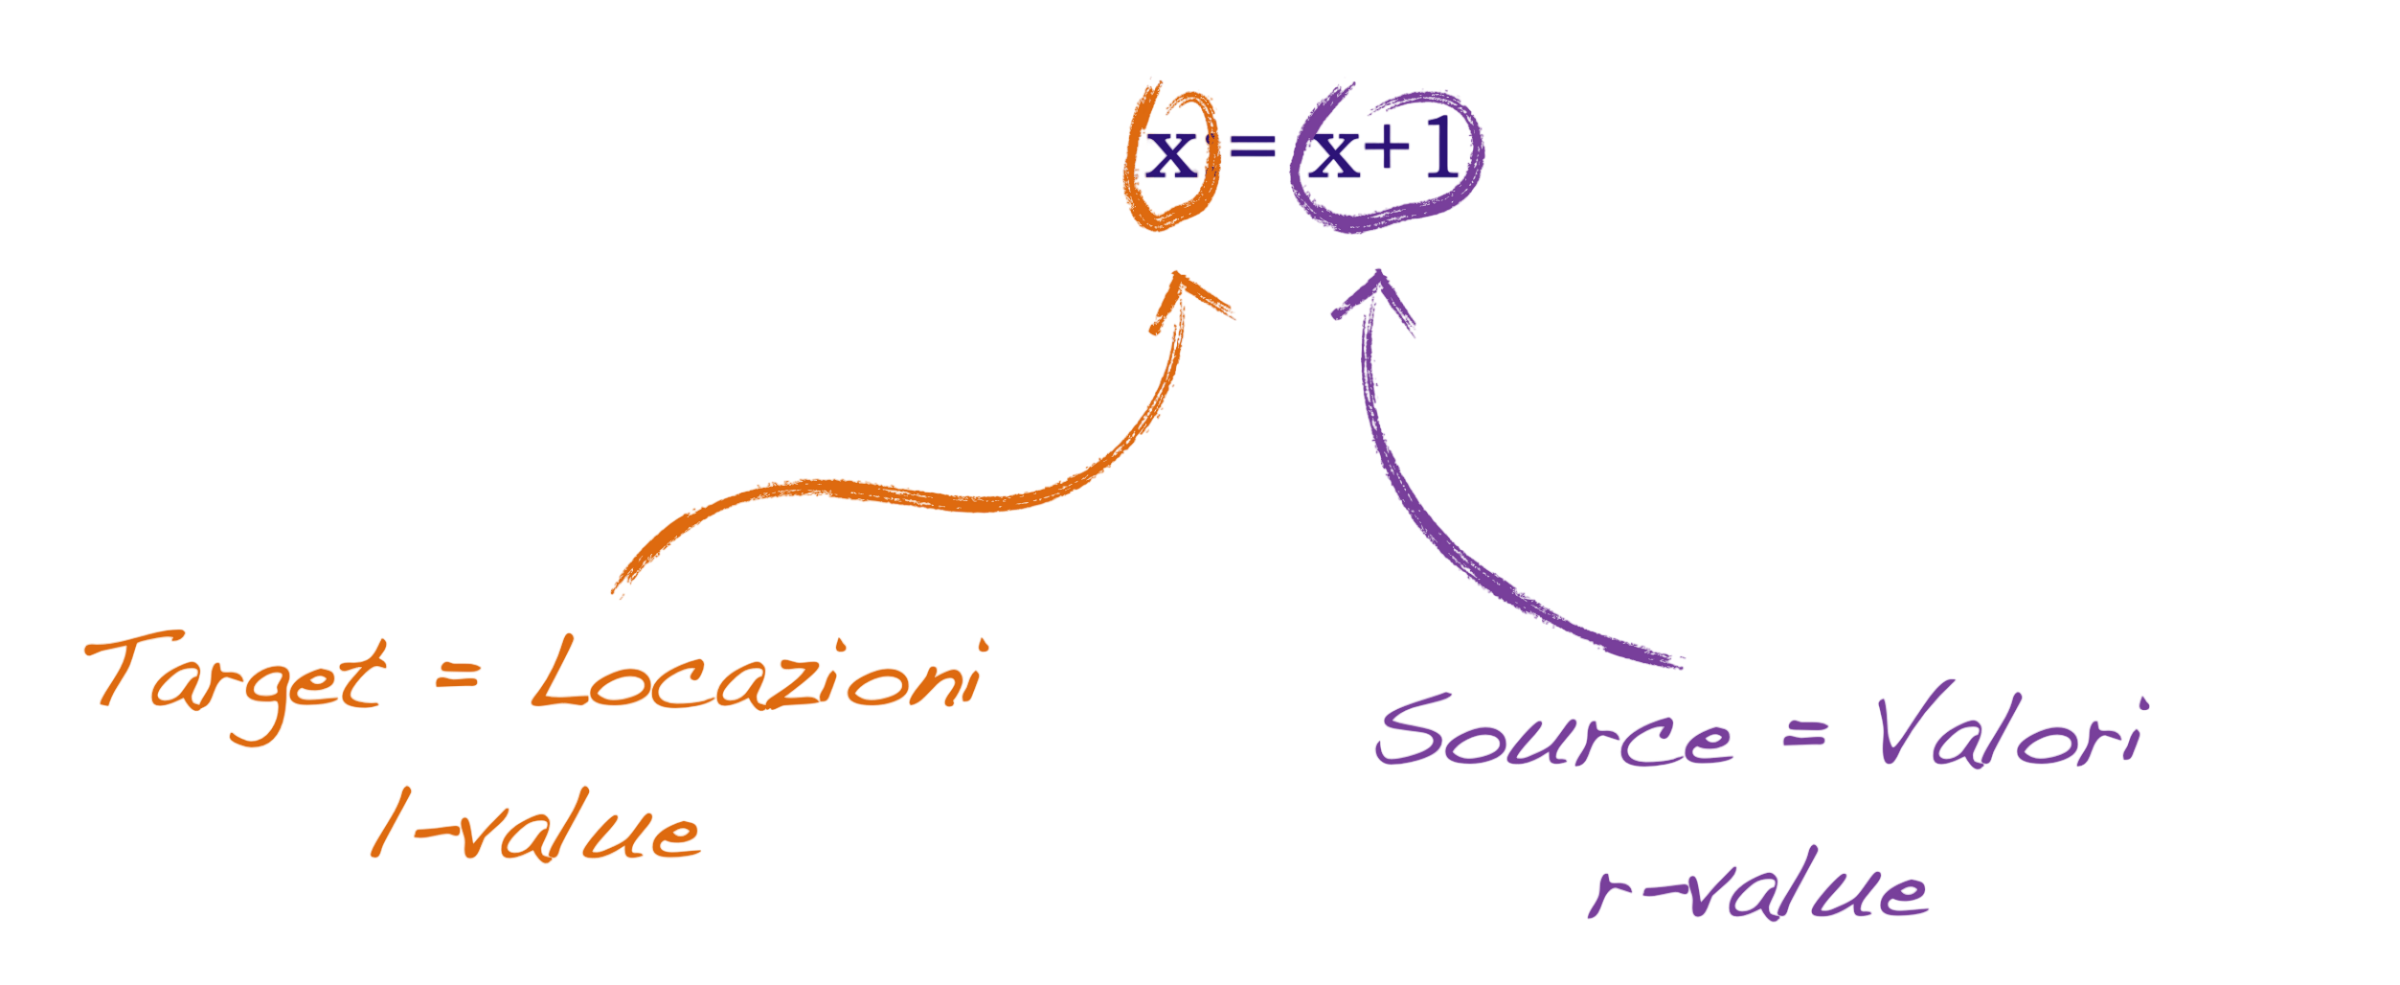
\includegraphics[width=0.55\textwidth]{images/assegnamento.png}
\end{figure}

\section{Semantica}
Definiamo gli identificatori liberi e definiti:
\[
    \begin{aligned}
        \mathrm{FI}(\texttt{x := e}) &= \mathrm{FI(\texttt{e})} \cup \{\mathrm{x}\}\\
        \mathrm{DI(\texttt{x := e})} &= \emptyset 
    \end{aligned}
\]

\subsection{Semantica statica}
La semantica statica per i comandi serve solo a verificare che il comando sia ben formato, ovvero rsipetti tutti i vincoli semantci del comando.\\[0.2ex]
Con la seguente notazione diciamo che il comando \texttt{c} è ben formato nell'ambiente statico $\Delta$, definito sull'insieme di identificatori $\mathrm{V}$:
\[
    \mathbf{\Delta \vdash_V c}
\]

L'assegamento è ben formato se l'identificatore a sinistra del simbolo di assegnamento è un identificatore variabile, e se è del tipo dell'espressione assegnata.\\[0.2ex]
Dobbiamo, quindi, valutare il tipo $\tau$ dell'espressione nello stesso ambiente statico e questo deve coincidere con il tipo associato dall'ambiente all'identificatore, che deve essere $\tau\text{loc}$.

\vario{Regola $\mathcal{C}_{\mathrm{S}_0}$}{
    \[
        \mathcal{C}_{\mathrm{S}_0}: \ \vdash \texttt{skip} \text{ (nessun vincolo da rispettare)}
    \]
}

\vario{Regola $\mathcal{C}_{\mathrm{S}_1}$}{
    \[
        \mathcal{C}_{\mathrm{S}_1}:\;
        \begin{prooftree}
            \hypo{\Delta \vdash_\mathrm{V} \mathrm{e} : \tau}
            \infer1{\Delta \vdash_\mathrm{V} \mathrm{x} := \tau}
        \end{prooftree}
        \quad \Delta(x) = \tau\text{loc}
    \]
}

\esempio{semantica statica}{

}


\subsection{Semantica dinamica}
Per la semantica dinamica dobbiamo valutare, per prima cosa, l'espressione.

\vario{Regola $\mathcal{C}_1$}{
    \[
        \mathcal{C}_1:\;
        \begin{prooftree}
            \hypo{\rho \vdash_\Delta \langle \mathrm{e}, \sigma \rangle \to_\mathrm{e} \langle \mathrm{e}', \sigma \rangle}
            \infer1{\rho \vdash_\Delta \langle \texttt{x := e}, \sigma \rangle \to_\mathrm{c} \langle \texttt{x := e'}, \sigma \rangle}
        \end{prooftree}
    \]
}

Una volta che l'espressione è completamente valutata, possiamo aggiornare la memoria associando a \texttt{x} il nuovo valore ottenuto e restituire, quindi, la memoria come configurazione terminale.

\vario{Regola $\mathcal{C}_2$}{
    \[
        \mathcal{C}_2 : \rho \vdash \langle \texttt{x := k}, \sigma \rangle    \to_\mathrm{c} \sigma[l \gets k] \quad \rho(\mathrm{x}) = 1
    \]
}

\esempio{semantica dinamica}{

}

\section{Strutture di controllo}

\subsection{Comandi di selezione}
I comandi di selezione forniscono gli strumenti per sceggliere tra due o più cammini di esecuzione:
\begin{itemize}[label=$\triangleright$, itemsep=\smallskipamount]
    \item \textbf{selettori a due vie} (\texttt{if-then-else})
    \item \textbf{selettori a più vie} (\texttt{switch-case})
\end{itemize}

\subsubsection{Selettori a due vie}
I comandi condizionali presentano la seguente sintassi:
\begin{bnfcode}{Sintassi comandi condizionali}
    if B then C else C
\end{bnfcode}

Prima, però, vediamo in che posizione si trovano gli identificatori dentro questo costrutto:
\[
    \begin{aligned}
        \mathrm{FI}(\texttt{if B then C else C}) &= \mathrm{FI}(\texttt{B}) \cup \mathrm{FI}(\texttt{C}) \cup \mathrm{FI}(\texttt{C})\\
        \mathrm{DI}(\texttt{if B then C else C}) &= \mathrm{DI}(C) \cup \mathrm{DI}(\texttt{C})
    \end{aligned}
\]

\paragraph{Semantica statica}
La semantica statica deve verificare se il comando è ben formato.\\[0.2ex]
In questo caso i vincoli da verificare saranno che l'espressione sia di tipo booleano e che i comandi dei rami condizionali siano ben formati.

\vario{Regola $\mathcal{C}_{\mathrm{S}_2}$}{
    \[
        \mathcal{C}_{\mathrm{S}_2}:\;
        \begin{prooftree}
            \hypo{\Delta \vdash_\mathrm{V} \ \texttt{e : bool} \quad \Delta \vdash_\mathrm{C} \mathrm{c}_0 \quad \Delta \vdash_\mathrm{V} \mathrm{c}_1}
            \infer1{\Delta \vdash_\mathrm{V} \texttt{if e then } \mathrm{c}_0 \texttt{ else } \mathrm{c}_1}
        \end{prooftree}
    \]
}

\esempio{semantica statica}{

}

\paragraph{Semantica dinamica}
La semantica dinamica valuta l'espressione di guardia e se questa è \texttt{true}, allora si scieglie di proseguire l'esecuzione con $\mathrm{c}_0$, altrimenti si prosegue con $\mathrm{c}_1$.

\vario{Regola $\mathcal{C}_3$}{
    \[
        \mathcal{C}_3:\;
        \begin{prooftree}
            \hypo{\rho \vdash_\Delta \langle \mathrm{B}, \sigma \rangle \to^*_\mathrm{e} \texttt{true}, \sigma \rangle}
            \infer1{\rho \vdash_\Delta \langle \texttt{if B then C else C}, \sigma \rangle \to_\mathrm{c} \langle \texttt{if true then $c_1$ else $c_2$}, \sigma\rangle}
        \end{prooftree}
    \]
}

\vario{Regola $\mathcal{C}_4$}{
    \[
        \mathcal{C}_4 : \rho \vdash_\Delta \langle \texttt{if true then $c_0$ else $c_1$}, \sigma \rangle \to_\mathrm{c} \langle c_0, \sigma \rangle
    \]
}

\vario{Regola $\mathcal{C}_5$}{
    \[
        \mathcal{C}_5 : \rho \vdash_\Delta \langle \texttt{if false then $c_0$ else $c_1$}, \sigma \rangle \to_\mathrm{c} \langle c_0, \sigma \rangle
    \]
}

\esempio{semantica dinamica}{

}


\subsubsection{Selettori a più vie}

\subsection{Composizione}
Prima di aggiungere altri comandi, abbiamo bisogno di comporre comandi in modo sequenziale.

\smallskip
La composizione sequenziale, donotata dal "\texttt{;}" permette di specificare in modo diretto la composizione di comandi deontando il fatto che il comando a destra del simbolo di composizione inizia dopo che il comando a sinistra ha completato l'esecuzione.
\[
        \mathbf{C ; C}
\]

La composizione non altera gli identificatori in posizione sia di definizione che liberi, che, quindi, saranno l'unione di quelli dei comandi:
\[
    \begin{aligned}
        \mathrm{FI}(\texttt{$\mathrm{c_0}$ ; $\mathrm{c_1})$} &= \mathrm{FI(c_0)} \cup \mathrm{FI(c_1)}\\
        \mathrm{FI(\texttt{$\mathrm{c_0}$ ; $\mathrm{c_1}$})} &= \mathrm{DI(c_0)} \cup \mathrm{DI(c_1)}
    \end{aligned}
\]

\subsubsection{Semantica statica}
Per la semantica statica si verifica che i comandi composti siano ben formati.

\vario{Regola $\mathcal{C}_{\mathrm{S}_3}$}{
    \[
        \mathcal{C}_{\mathrm{S}_3}:\;
        \begin{prooftree}
            \hypo{\Delta \vdash_\mathrm{V} \mathrm{c}_0 \quad \Delta \vdash_\mathrm{V} \mathrm{c}_1}
            \infer1{\Delta \vdash_\mathrm{V} \mathrm{c}_0 : \mathrm{c}_1}
        \end{prooftree}
    \]
}

\vario{Regola $\mathcal{C}_{\mathrm{S}_4}$}{
    \[
        \mathcal{C}_{\mathrm{S}_4} : \Delta \vdash_\mathrm{V} \texttt{skip}
    \]
}

\subsubsection{Semantica dinamica}
Per la semantica dinamica, lo \texttt{skip} lasca inalterata la memoria, mentre la compozione esegue $\mathrm{c}_0$ e poi a partire dalla memoria risultante esegue $\mathrm{c}_1$.

\vario{Regola $\mathcal{C}_6$}{
    \[
        \mathcal{C}_6 : \rho \vdash_\Delta \langle \texttt{skip}, \sigma \rangle \to_\mathrm{c} \sigma
    \]
}

\vario{Regola $\mathcal{C}_7$}{
    \[
        \mathcal{C}_7:\;
        \begin{prooftree}
            \hypo{\rho \vdash_\Delta \langle \mathrm{c}, \sigma \rangle \to_\mathrm{c} \langle \mathrm{c}', \sigma \rangle}
            \infer1{\rho \vdash_\Delta \langle \mathrm{c} ; \mathrm{c}_0, \sigma \rangle \to_\mathrm{c} \langle \mathrm{c}' ; \mathrm{c}_0, \sigma \rangle}
        \end{prooftree}
    \]
}

\vario{Regola $\mathcal{C}_8$}{
    \[
        \mathcal{C}_8:\;
        \begin{prooftree}
            \hypo{\rho \vdash_\Delta \langle \mathrm{c}, \sigma \rangle \to_\mathrm{c} \sigma'}
            \infer1{\rho \vdash_\Delta \langle \mathrm{c} ; \mathrm{c}_0, \sigma \rangle \to_\mathrm{c} \langle \mathrm{c}_0, \sigma' \rangle}
        \end{prooftree}
    \]
}

\subsection{Comandi iterativi}
L'iterazione e la ricorsione sono due meccanismi che permettono di ottenere formalismi di calcolo di Turing completi, senza di essi avremmo solo automi a stati finiti.

\smallskip
In genrale, si parla di \textbf{iterazione indeterminata} quando i cicli sono controllati logicamente, ovvero su un'espressione booleana (\texttt{while, repeat, ...}).\\[0.2ex]
Si parla, invece, di \textbf{iterazione determinata} quando i cicli sono controllati numericamente, con numero di ripetizioni del ciclo determinate al momento dell'inizio del ciclo (\texttt{for, do, ...}).

\smallskip
Vediamo per prima cosa in che posizione si trovano gli identificatori dentro questo costrutto:
\[
    \begin{aligned}
        \mathrm{FI(\texttt{while e do c})} &= \mathrm{FI(c)} \cup \mathrm{e}\\
        \mathrm{DI(\texttt{while e do c})} &= \mathrm{DI(c)}
    \end{aligned}
\]

\subsubsection{Semantica statica}
La semantia statica deve verificare se il comando è ben formato.\\[0.2ex]
In questo caso i vincoli da verificare saranno che l'espressione sia di tipo booleano e che il comando nel corpo sia ben formato.

\vario{Regola $\mathcal{C}_{\mathrm{S}_5}$}{
    \[
        \mathcal{C}_{\mathrm{S}_5}:\;
        \begin{prooftree}
            \hypo{\Delta \vdash_\mathrm{V} \ \texttt{e : bool} \quad \Delta \vdash_\mathrm{V} \mathrm{c}}
            \infer1{\Delta \vdash_\mathrm{V} \texttt{while e do c}}
        \end{prooftree} 
    \]
}

\subsubsection{Semantica dinamica}

\vario{Regola $\mathcal{C}_9$}{
    \[
        \mathcal{C}_9:\;
        \begin{prooftree}
            \hypo{\rho \vdash_\Delta \langle \mathrm{e}, \sigma \rangle \to^*_\mathrm{e} \langle \texttt{true}, \sigma \rangle}
            \infer1{\rho \vdash_\mathrm{\Delta} \langle \texttt{while e do c}, \sigma \rangle \to_\mathrm{c} \langle \texttt{c ; while e do c}, \sigma \rangle}
        \end{prooftree}
    \]
}

\vario{Regola $\mathcal{C}_{10}$}{
    \[
        \mathcal{C}_{10}:\;
        \begin{prooftree}
            \hypo{\rho \vdash_\Delta \langle \mathrm{e}, \sigma \rangle \to^*_\mathrm{e} \langle \texttt{false}, \sigma \rangle}
            \infer1{\rho \vdash_\mathrm{\Delta} \langle \texttt{while e do c}, \sigma \rangle \to_\mathrm{c} \sigma}
        \end{prooftree}
    \]   
}

    %!Tex root = Linguaggi.tex

\chapter{Procedure}
L'uso delle procedure permette l'\textbf{astrazione del controllo}.

\vario{Nota}{
    Astrarre significa nascondere dettagli facendo emergere caratteristcihe comuni.
}

L'astrazione chiede di identificare le proposizioni importanti che si vuole descrivere al fine di concentrarsi che si vuole descrivere al fine di concentrarsi sulle questioni rilvanti e ignorare quelle non importanti.

\smallskip
Quando si parla di astrazione del controlllo ci sono, in realtà, due categorie di sottoprogrammi con nome nome che possiamo definire:
\begin{itemize}[label=$\diamond$, itemsep=\smallskipamount]
    \item \textbf{procedure} (no output)
    \item \textbf{funzioni} (restituisce output)
\end{itemize}

\smallskip
Partre importante del processo di astrazione consiste nel dare al raggruppamento un nome.\\[0.2ex]
Il \textbf{nome} permette di rifersi all'astrazione senza conoscerne i dettagli, una solo le caratteristiche di interesse che ne hanno determinato il raggruppamento.\\[0.2ex]
I \textbf{parametri} permettono l'astrazione di tante computazioni simili che cambiano di tante computazioni simili che cambiano solo per alcuni input a cui vengono applicate e che vengono abbreviate con un singolo nome.\\[0.2ex]
Il \textbf{corpo} è ciò che viene valutato/eleborato/eseguito ogni volta che il nome viene richiamato.

\smallskip
Una procedura viene definita in tre fasi:
\begin{enumerate}[itemsep=\smallskipamount]
    \item \textbf{specifica}: descrizione dell'interfaccia della procedura/funzione
    \begin{lstlisting}[language=C]
        double P(int x) {
            
        }
    \end{lstlisting}
    \item \textbf{definizione}: descrizione del copro della procedura/funzione
    \begin{lstlisting}[language=C]
        {
            double y;
            //corpo procedura P
            ...
            (return y);
        }
    \end{lstlisting}
    \item \textbf{uso}: chiamata della procedura/funzione per eseguire il codice
    \begin{lstlisting}[language=C]
        int n;
        double z;
        z = P(n); //chiamata della procedura
    \end{lstlisting}
\end{enumerate}

Consideriamo il seguente codice:
\begin{lstlisting}[language=C, caption=programma di esempio]
    int foo(int n) {
        int tmp = a;

        if(tmp == 0)
            return n;
        else
            return n + 1;
    }
\end{lstlisting}

In questo caso la variabile \texttt{a} è un identificatore non locale, cioè un identificatore libero per cui di deve trovare il significato nel contesto.
\end{document}